%%%%%%%%%%%%%%%%%%%%%%%%%%%%%%%%%%%%%%%%%%
% labInstructions.cls provides all the styles needed
% us the option 'full' to show the solutions and
% additional assistant informations
%%%%%%%%%%%%%%%%%%%%%%%%%%%%%%%%%%%%%%%%%%
\documentclass[full]{labInstructions}

\ifthenelse{\boolean{showAdditional}}{
\title{{\Huge \scshape Laboratoire de physique des particules}\\\vspace{0.5cm}{\Large Laboratoire PHYS-F-311 -- \textit{Version Assistants}}}}
{\title{{\Huge \scshape Laboratoire de physique des particules}\\\vspace{0.5cm}{\Large Laboratoire PHYS-F-311}}}

\author{Author list to be defined...}
\date{\today}

\begin{document}

\maketitle
\thispagestyle{empty}
\setcounter{tocdepth}{2}
\tableofcontents
\setcounter{page}{1}
\vspace{3cm}
\ifthenelse{\boolean{showAdditional}}{
\begin{additional}
\textbf{Attention!}\\
Cette version contient des informations supplémentaires destinées aux assistants. Celles-ci sont indiquées par une barre grise située sur le côté gauche.
\end{additional}
}

%%%%%%%%%%%%%%%%%%%%%%%%%%%%%%%%%%%%%%%%%%
% Introduction
%%%%%%%%%%%%%%%%%%%%%%%%%%%%%%%%%%%%%%%%%%
\section{Introduction}

Cette manipulation a pour but la caract\'erisation d'un module optique (OM) développé pour l'expérience AMANDA. Afin d'étidier les propriétés de cet OM, vous devrez mettre au point le dispositif nécéssaire à la prise de mesure. Après avoir pris connaissance avec le dispositif, vous serez ainsi amené à développer vous même la logique d'acquisition des données. Vous analyserez ensuite celle-ci grâce au outils statistiques et informatiques que vous aurez vous en cours. 

\pagebreak


%%%%%%%%%%%%%%%%%%%%%%%%%%%%%%%%%%%%%%%%%%
% Common description of the materials
%%%%%%%%%%%%%%%%%%%%%%%%%%%%%%%%%%%%%%%%%%
\section{Le matériel expérimental}

\subsection{Scintillateurs}

\subsection{Photo-multiplicateurs}

\begin{figure}
    \centering
	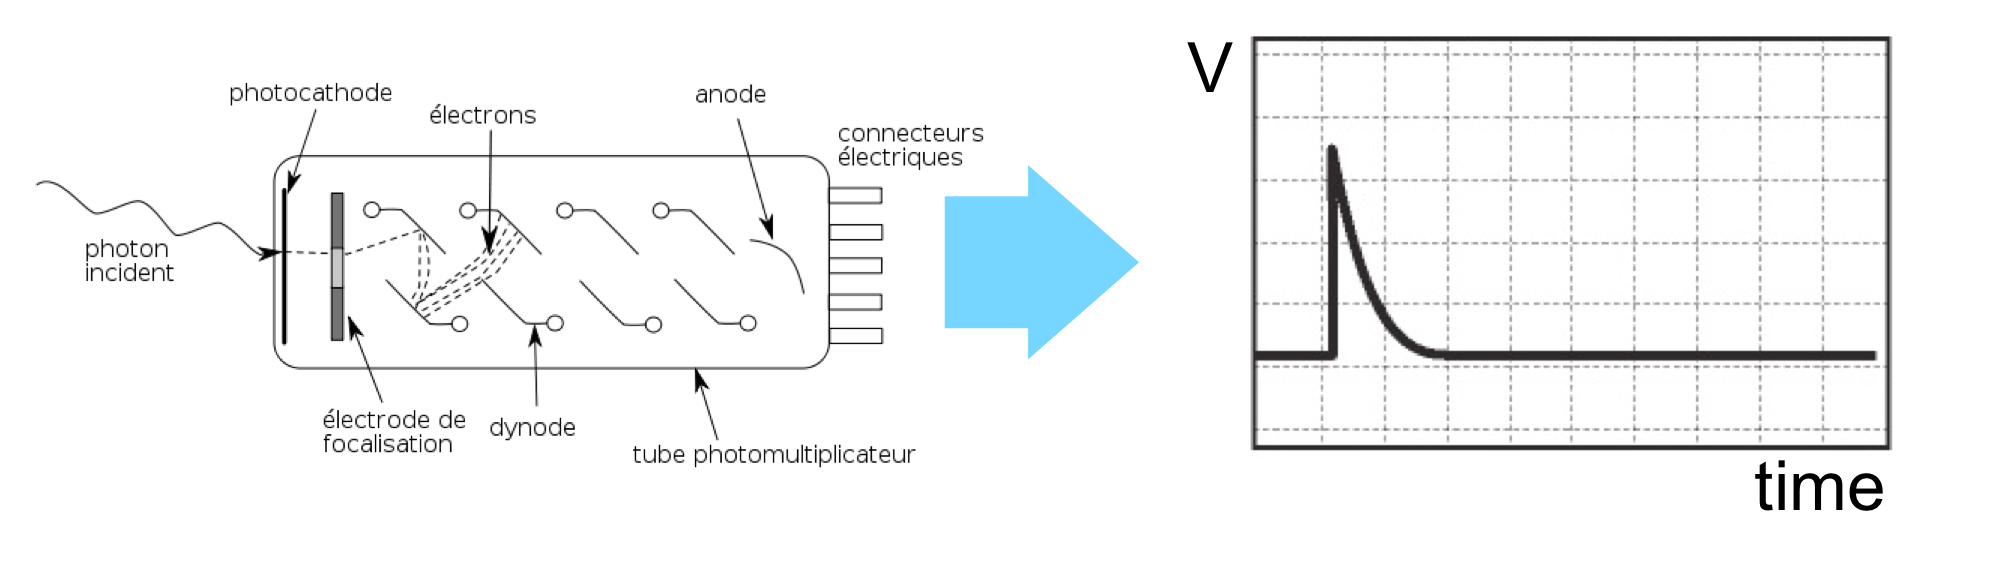
\includegraphics[width=\textwidth]{figures/PMT_readout.png}
    \caption{Schema du fonctionnement d'un photo-multiplicateur(PMT).}
    \label{fig:PMT_readout} 
\end{figure}

Nous allons à présent étudier les différentes composantes d'un spectre en charge typique de la réponse d'un photo-multiplicateur.\\

\begin{figure}[!h]
    \center{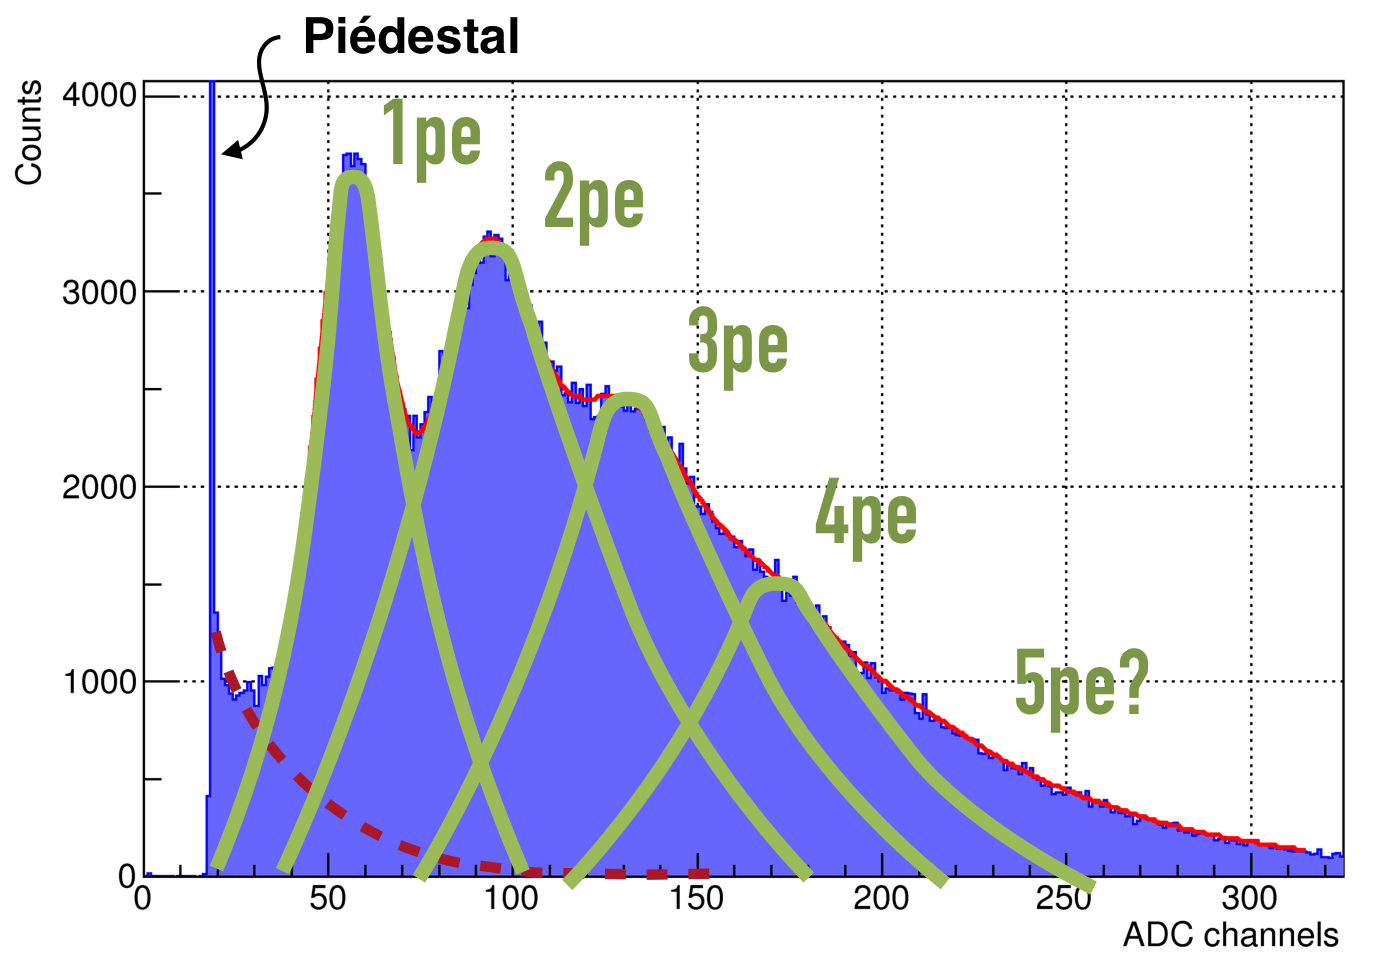
\includegraphics[width=0.7\textwidth]
    {figures/SpectreEnCharge.png}}
    \caption{\label{fig:spectre} Spectre en charge d'un photo-multiplicateur.}
\end{figure}

\textbf{Piédestal :} Il s'agit d'évènements sans charge qui prennent la forme d'un pic en zéro. Afin de se débarrasser de cet effet, il vous faudra régler au mieux votre seuil.\\

\textbf{Dark current :} Il s'agit de bruit associé au PM, il survient lorsqu'un électron est arraché à une dynode sans qu'un photon incident n'arrive à la photo-cathode. Il nous donne une exponentielle décroissante. Cet effet est exacerbé lorsque la tension aux bornes du photo-multiplicateur est élevée. \\

\textbf{Pic des photo-électrons :} Ce sont le réponse en charge du PM pour différent nombre de photo-électrons.\\

Le largeur de la gaussienne du premier photo-électron (1pe) va nous donner la résolution en charge du PM. La relation entre la hauteur des gaussiennes nous est donné par la distribution de Poisson.

\subsection{Aquisition de donn{\'e}es}

\begin{figure}
    \centering
    \begin{subfigure}[t]{0.2\textwidth}
        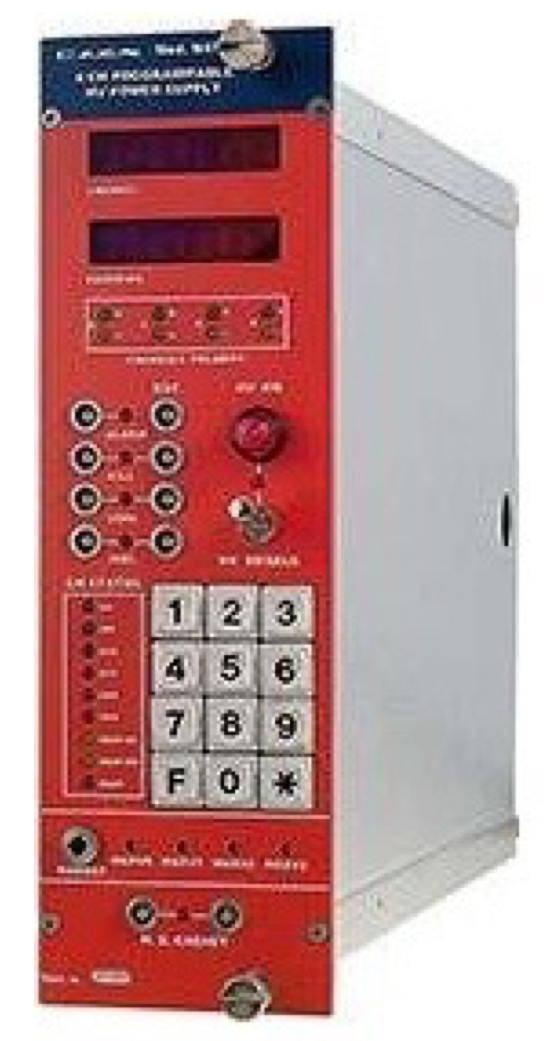
\includegraphics[height=0.25\textheight, width=\textwidth, keepaspectratio]{figures/Alim1.png}
        \caption{Alimentation de haute tension}
        \label{fig:HV1}
    \end{subfigure}
    \hfill
    \begin{subfigure}[t]{0.2\textwidth}
        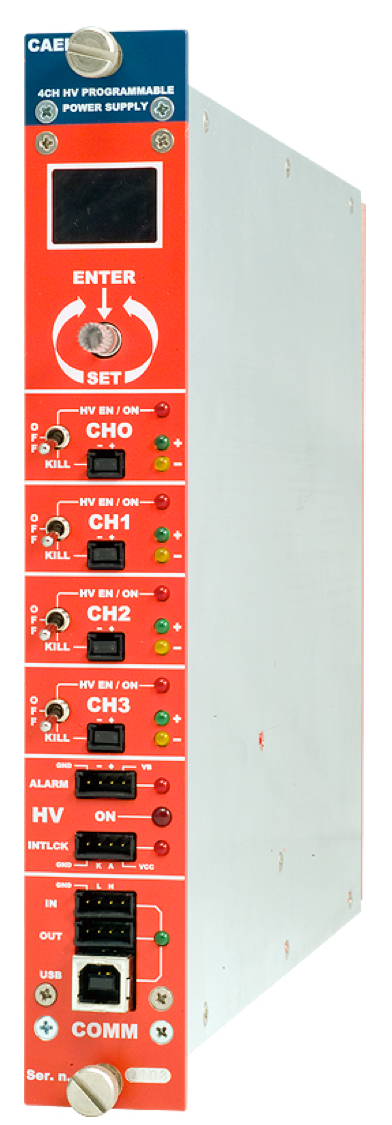
\includegraphics[height=0.25\textheight, width=\textwidth, keepaspectratio]{figures/Alim2.png}
        \caption{Alimentation de haute tension}
        \label{fig:HV2}
    \end{subfigure}
    \hfill
    \begin{subfigure}[t]{0.2\textwidth}
        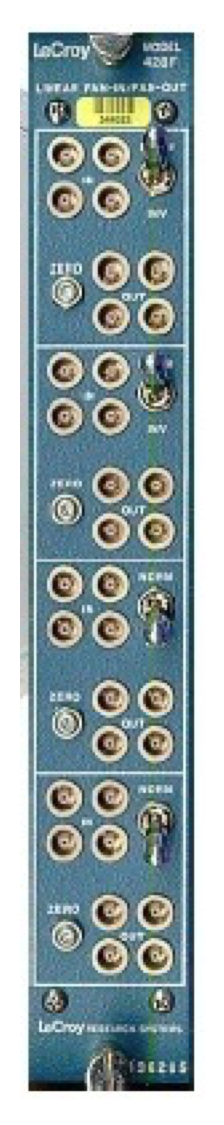
\includegraphics[height=0.25\textheight, width=\textwidth, keepaspectratio]{figures/FanInFanOut.png}
        \caption{Distributeur de signal \emph{fan-in-fan-out}}
        \label{fig:fifo}
    \end{subfigure}
    \hfill
    \begin{subfigure}[t]{0.2\textwidth}
        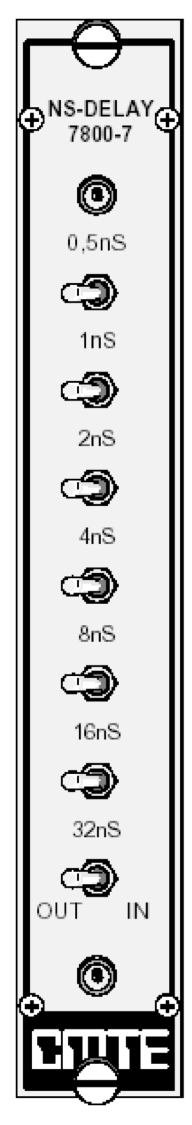
\includegraphics[height=0.25\textheight, width=\textwidth, keepaspectratio]{figures/delay.png}
        \caption{Delayeur de signal}
        \label{fig:delay}
    \end{subfigure}
    
	\vspace{1cm}
    \begin{subfigure}[t]{0.2\textwidth}
        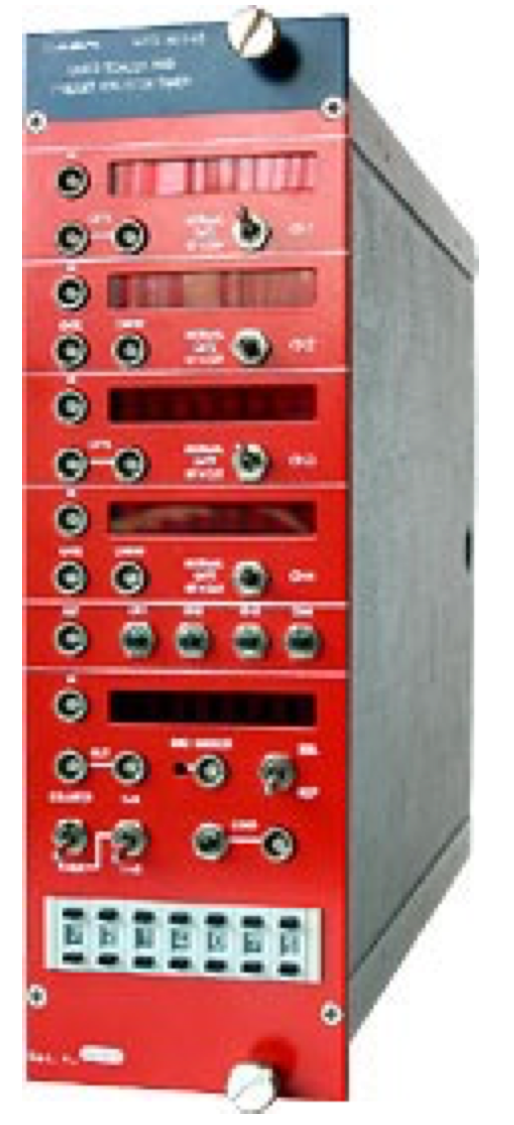
\includegraphics[height=0.25\textheight, width=\textwidth, keepaspectratio]{figures/scaler.png}
        \caption{Scaler NIM}
        \label{fig:scaler1}
    \end{subfigure}
    \hfill
    \begin{subfigure}[t]{0.25\textwidth}
        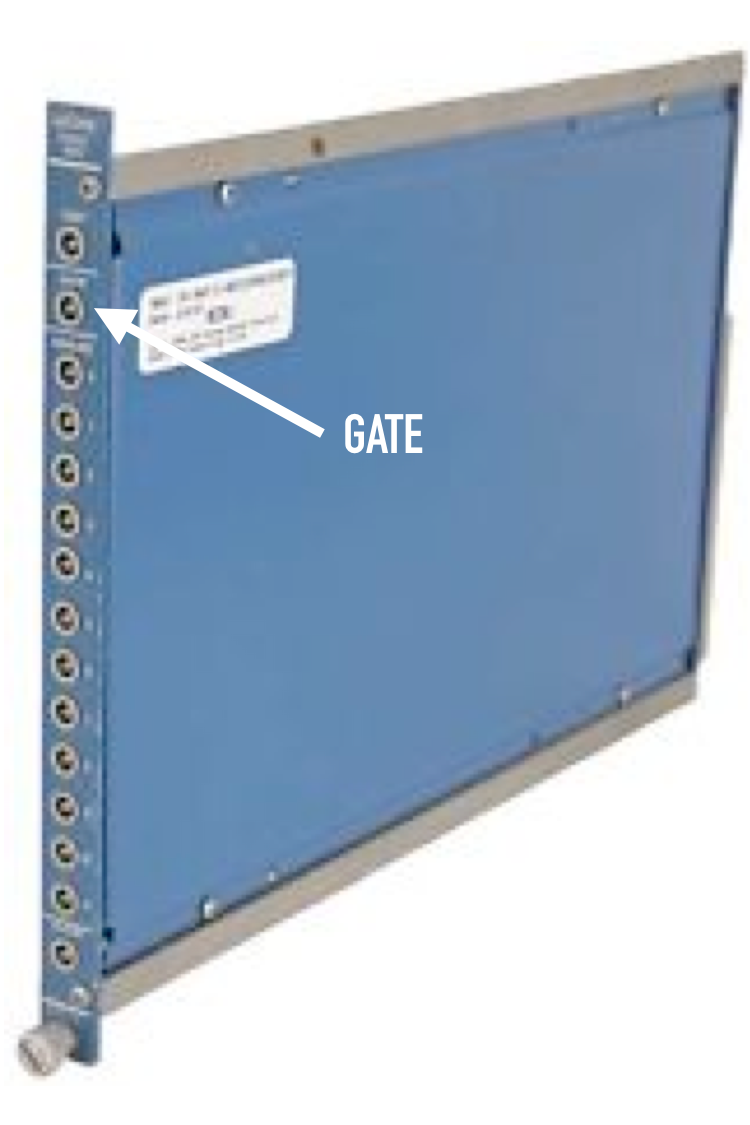
\includegraphics[height=0.25\textheight, width=\textwidth, keepaspectratio]{figures/gate.png}
        \caption{Scaler CAMAC}
        \label{fig:scaler2}
    \end{subfigure}    
    \hfill
    \begin{subfigure}[t]{0.45\textwidth}
        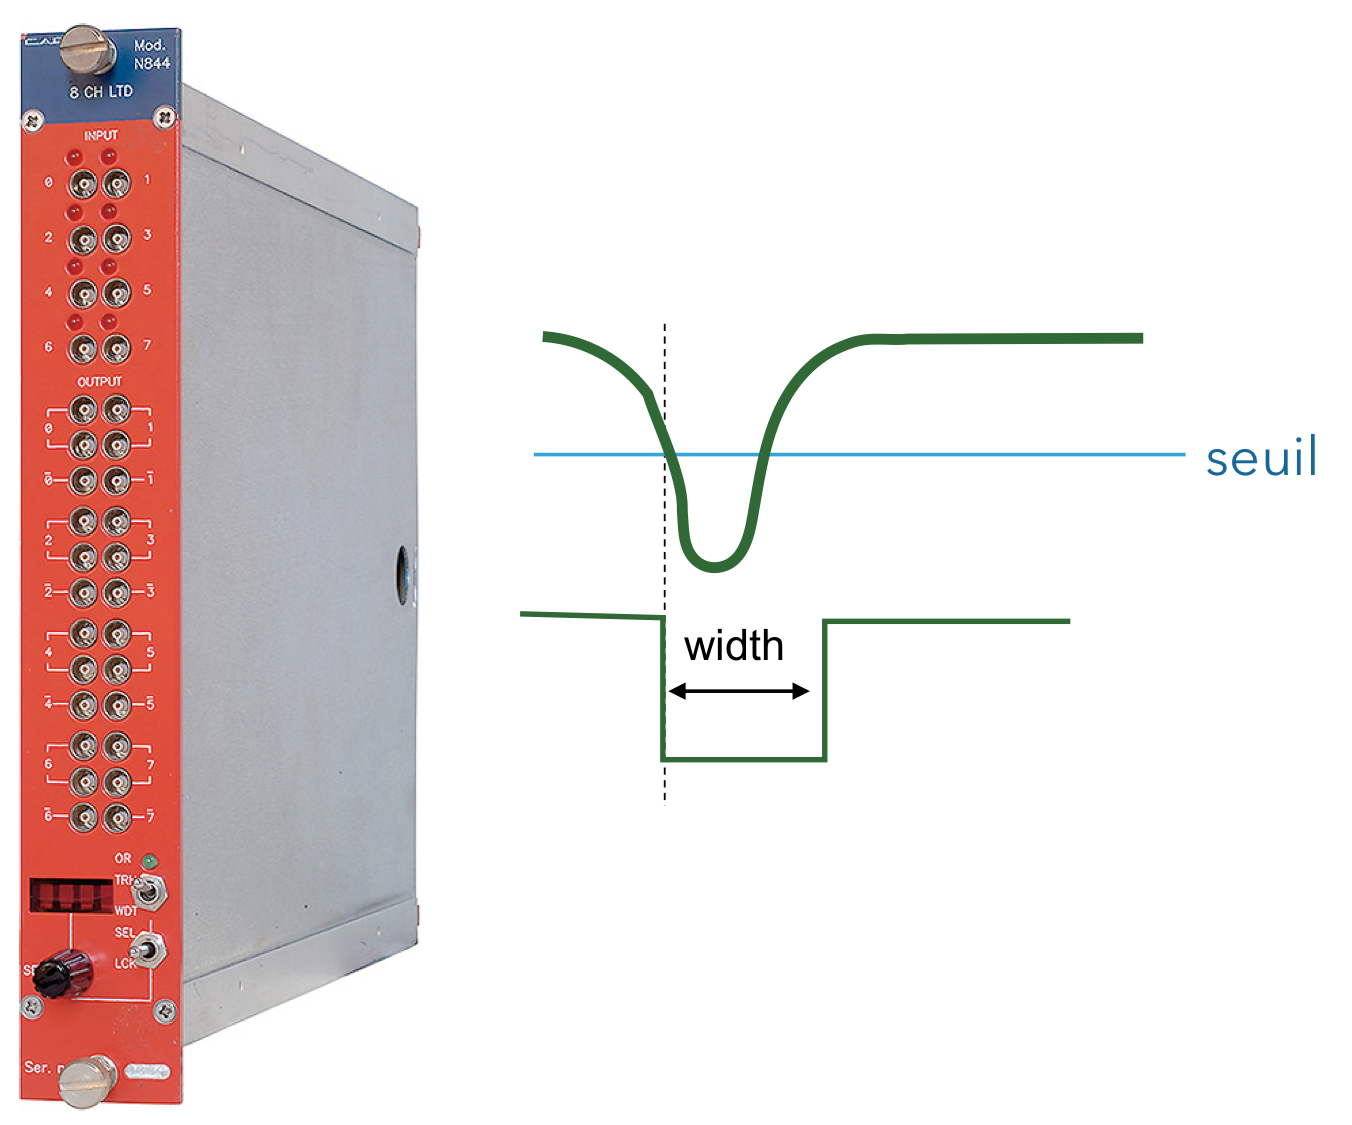
\includegraphics[height=0.3\textheight, width=\textwidth, keepaspectratio]{figures/Discriminateur.png}
        \caption{Discriminateur}
        \label{fig:discriminator}
    \end{subfigure}

	\vspace{1cm}    
    \begin{subfigure}[t]{0.45\textwidth}
        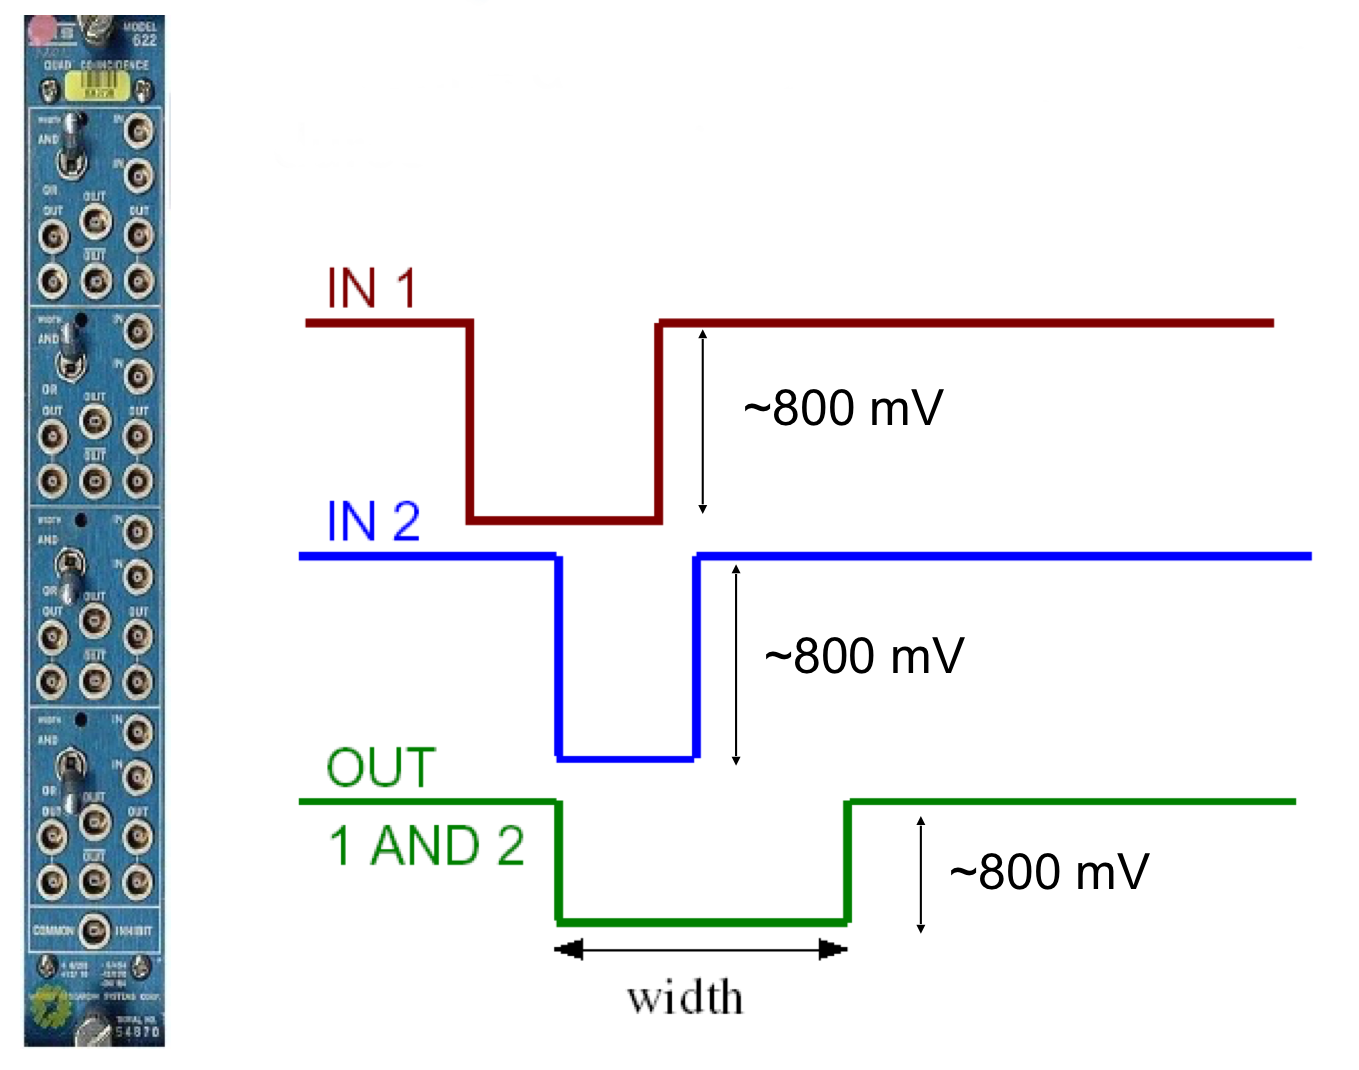
\includegraphics[height=0.3\textheight, width=\textwidth, keepaspectratio]{figures/UniteDeCoincidence_crop.png}
        \caption{Unit{\'e} de co{\"i}ncidence}
        \label{fig:coincidence}
    \end{subfigure}
    \hfill
    \begin{subfigure}[t]{0.45\textwidth}
        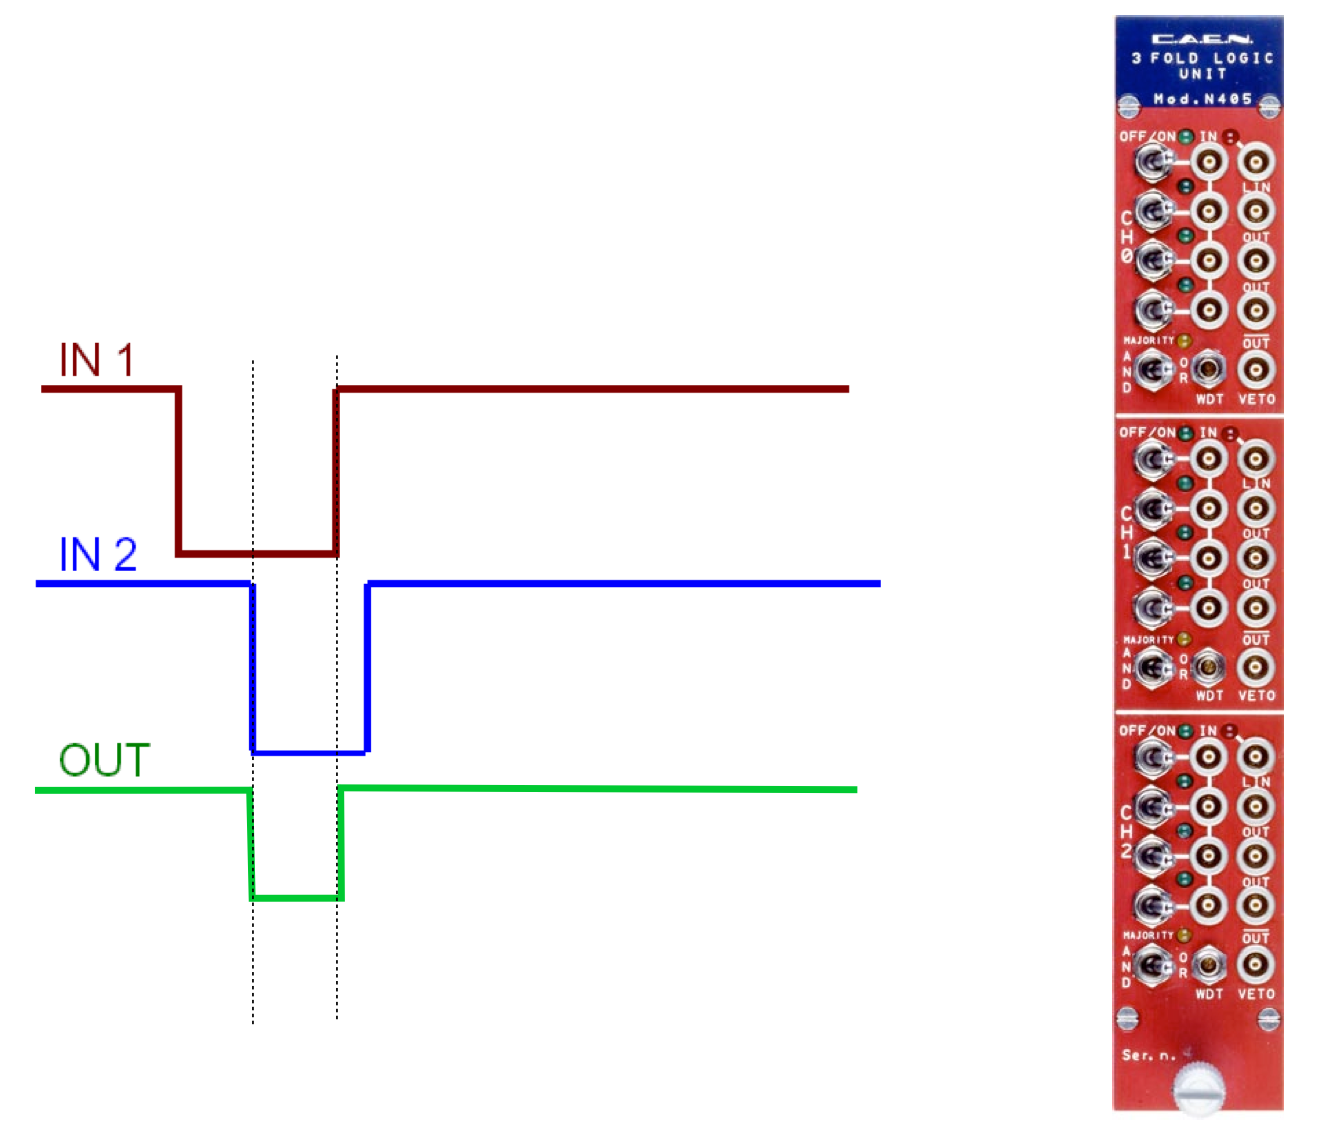
\includegraphics[height=0.3\textheight, width=\textwidth, keepaspectratio]{figures/UniteLogiqueProgrammable.png}
        \caption{Unit{\'e} logique programmable}
        \label{fig:plu}
    \end{subfigure}
    \caption{Appareils utilis{\'e}s dans les dispositifs.}
    \label{fig:devices}
\end{figure}

%%%%%%%%%%%%%%%%%%%%%%%%%%%%%%%%%%%%%%%%%%
% Brief intro to statistics
%%%%%%%%%%%%%%%%%%%%%%%%%%%%%%%%%%%%%%%%%%
\section{Methodes d'analyse statistique}

Au cours de ce laboratoire, il vous faudra analyser les données que vous aurez recueillies. Pour cela, vous aurez à votre disposition plusieurs iPython Notebook que vous étudierez en profondeur lors du cours de statistique. Ces différents outils sont accessibles via le lien suivant:\\
\url{https://github.com/zemrude/PHYS-F-311}

\subsection{Méthode Monte Carlo}
Afin de développer votre méthode d'ajustement, il vous sera demandé, dans un premier temps,  de créer un ensemble de données que vous générerez via la technique de simulation Monte Carlo (MC). Vous avez à votre disposition deux méthodes pour générer vos données: la transformation inverse et le "Hit and Miss". A l'aide de ces deux techniques, vous serez en mesure de générer des évènements aléatoire suivant la distribution de votre choix (gaussienne, loi exponentielle, ...).

\subsubsection{Hit $\&$ Miss}
La méthode Hit $\&$ Miss ou méthode du rejet consiste à générer aléatoirement un grand nombre d'évènements et à ne sélectionner ensuite que ceux remplissant les conditions pré-établies, i.e. les évènements sous la courbe de la distribution choisie. 

\begin{figure}[h!]
\center{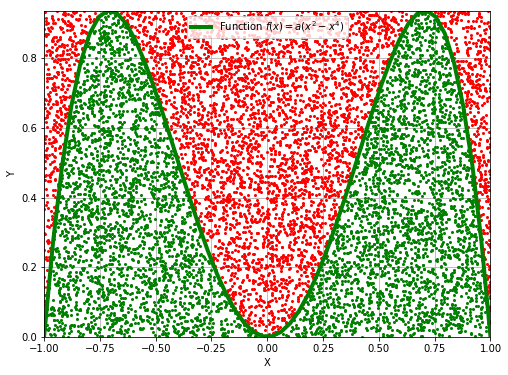
\includegraphics[width=0.6\textwidth]{figures/Hit_and_miss.png}}
\caption{Simulation obtenue par la méthode du Hit $\&$ Miss. Les points représentent les évènements générés aléatoirement. Les éléments en vert sont ceux qui ont remplissent la condition fixée pour suivre la distribution souhaitée. Les points rouges sont rejetés et auront donc été simulés en vain.}
\label{fig:HitMiss}
\end{figure}

Pour notre exemple illustré par la figure \ref{fig:Inverse}, la fonction $f(x)=a(x^{2}-x^{4})$ a été choisie. La figure \ref{fig:HitMiss} illustre la méthode du Hit $\&$ Miss en indiquant en vert les points qui sont sous la courbe de la distribution que l'on souhaite reproduire. Les points rouges seront rejetés. Cette méthode demande donc plus de ressources afin d'obtenir suffisamment de statistique puisqu'une partie des évènements générés ne  sera finalement pas utilisée.

\subsubsection{Transformation inverse}
A l'aide de cette méthode,  un échantillon aléatoire de nombres suivant une distribution donnée peut être directement produit. Les données aléatoires sont obtenues à partir de l'inverse de la fonction de répartition. Cette méthode se base sur le théorème de la réciproque. Dans un premier temps, il nous faut calculer l'inverse de notre fonction, $F(x)$, en fonction de $x$. Les évènements générés aléatoirement seront ensuite passé dans la fonction inverse afin d'obtenir la distribution souhaitée. 

\begin{figure}[h!]
\center{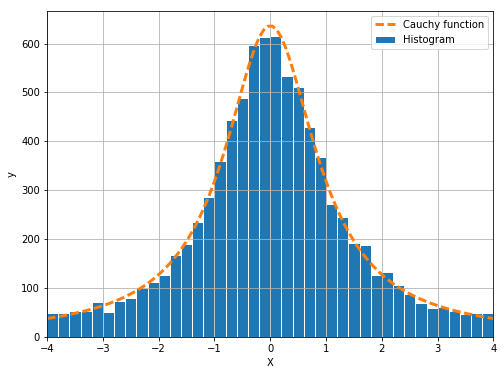
\includegraphics[width=0.6\linewidth]{figures/Inverse_transformation.png}}
\caption{Histogramme des évènements générés par la méthode de transformation inverse pour la distribution de Cauchy.}
\label{fig:Inverse}
\end{figure}

Pour notre exemple illustré par le graphique \ref{fig:Inverse}, nous allons considérer la loi de Cauchy, dont la fonction de répartition s'écrit:

\begin{equation}
F(x) = \frac{1}{2} + \frac{1}{\pi} \arctan \left(\frac{x - x_{0}}{a}\right) \, .
\end{equation}

On a alors:

\begin{equation}
u = F(x) \Longleftrightarrow x = x_{0} + a \tan \left[ \pi  \left(u - \frac{1}{2} \right)  \right] \, .
\end{equation}

La simulation peut donc être obtenue en suivant :

\begin{equation}
X = x_{0} + a \tan \left[ \pi  \left(U - \frac{1}{2} \right)  \right] \, .
\end{equation}

La fonction de Cauchy est indiquée en orange alors que les données simulées obtenues à partir de notre méthode inverse sont mise en histogramme. On peut voir que la distribution de ces évènements reproduit correctement la loi de Cauchy.

\subsection{Ajustement}
Nous allons à présent développer la méthode d'ajustement sur les données que vous venez d'obtenir par la méthode Monte Carlo de votre choix. Deux méthodes vous sont à nouveau proposées pour ce "fit": la méthode des moindre carré ($\chi^2$) et la méthode du maximum de vraisemblance. Ces deux méthodes permettent de comparer nos données avec les prédictions théorique de notre modèle. Une fois au point, vous pourrez donc utiliser cet ajustement sur vos données réelles afin de confirmer que votre échantillon a bien le comportement attendu. 

\textbf{Remarque :} La minimisation n'est pas effectuée directement sur les données mais sur les données déjà représentées en histogramme.

\subsubsection{Moindre carré - $\chi^{2}$}
Considérons la distribution de nos évènements générés par MC  que l'on désire ajuster au mieux par une fonction $f(x)$ que nous choisirons de façon pertinente en fonction du phénomène étudier. Nous cherchons les paramètres de cette fonction minimisant la somme des carrés des distances entre la hauteur de nos barres d'histogrammes, $y_i$, en $x_i$ et $f(x_i)$, autrement dit:

\begin{equation}
\chi^2 = \sum_{i=1}^{N} \left[ y_i - f(x_i) \right]^2 \, .
\end{equation}

Pour notre exemple, nous considérons une distribution d'évènement suivant une décroissance exponentielle dont nous tentons de trouver le temps de vie, $\tau$. Notre fonction est donc donnée par:

\begin{equation}
f(x) = \alpha \exp(-x / \tau) \, .
\end{equation}

La valeur de $\tau$ minimisant $\chi^2$ est illustrée par la figure \ref{fig:chi2}. Celle-ci est utilisée pour l'ajustement de la figure de droite.

\begin{figure*}[h!]
    \centering
    \begin{minipage}[b]{0.48\linewidth}
    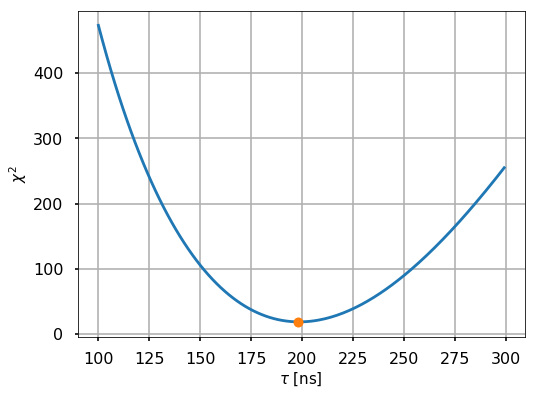
\includegraphics[width=\linewidth]{figures/chi_2.png}
    \end{minipage}
    \hfill
    \begin{minipage}[b]{0.51\linewidth}
    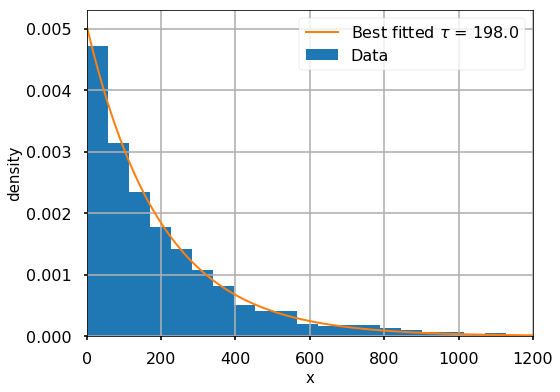
\includegraphics[width=\linewidth]{figures/chi_2_bestfit.png}
    \end{minipage}
    \caption{\textbf{Gauche :} La valeur de $\tau$ minimisant $\chi^2$ est désignée par le point orange. \textbf{Droite :} Le fit obtenu à partir de $\tau_{best}$ (orange) est mis en graphique au côté de la distribution des données MC que nous tentions d'ajuster.}
    \label{fig:chi2}
\end{figure*}

\subsubsection{Maximum de vraisemblance}
La méthode de maximum de vraisemblance est une méthode statistique nous permettant d'évaluer la valeur la plus "vraisemblable" des paramètres d'un modèle probabiliste. 

Pour notre exemple, nous considérons la loi normale exprimée comme suit:

\begin{equation}
f(x) = \frac{1}{\sigma\sqrt{2\pi}} \exp{-\frac{1}{2} \left( \frac{x-\mu}{\sigma}\right)^2} \,  , 
\end{equation}

où $\sigma$ est l'écart type et $\mu$ est la moyenne. Nous allons à présent tenter de trouver la valeur de $\mu$ optimisant la fonction de vraisemblance,  $\mathcal{L}$. Pour cela nous fixons l'écart type de la Gaussienne et laissons varier la moyenne. Nous trouvons ensuite la valeur de $\mu$ qui minimise $-\log{\mathcal{L}}$, comme illustré par la figure \ref{fig:MaxLikelihood}.

\begin{figure*}[h!]
    \centering
    \begin{minipage}[b]{0.49\linewidth}
    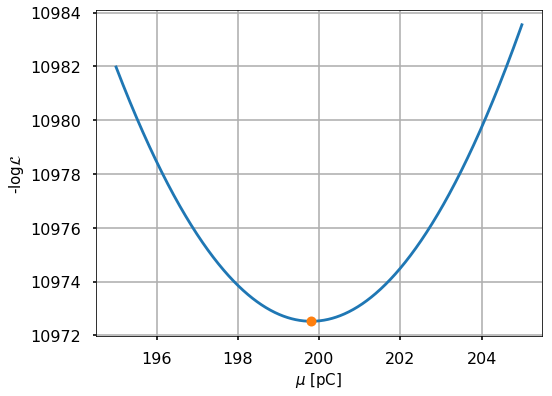
\includegraphics[width=\linewidth]{figures/MaxLikelihood.png}
    \end{minipage}
    \hfill
    \begin{minipage}[b]{0.49\linewidth}
    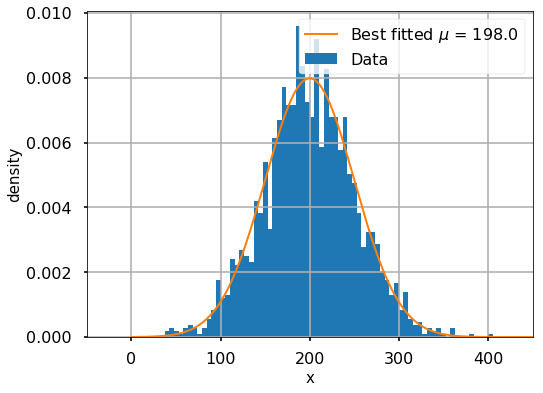
\includegraphics[width=\linewidth]{figures/MaxLikelihood_bestFit.png}
    \end{minipage}
    \caption{\textbf{Gauche :} La valeur de $\mu$ minimisant $-\log{\mathcal{L}}$ est désignée par le point orange. \textbf{Droite :} Le fit obtenu à partir de $\mu_{best}$ (orange) est mis en graphique au côté de la distribution des données MC que nous tentions d'ajuster.}
    \label{fig:MaxLikelihood}
\end{figure*}


\subsection{Erreur sur l'ajustement}
Nous pouvons également estimer l'erreur associée à une valeur ajustée. Nous allons pour cela faire varier de l'unité choisie (1, 2, 3, ...) la valeur minimale de la méthode choisie. Nous obtiendrons ainsi l'erreur en terme de $\sigma$. L'erreur sur le paramètre à ajuster nous indique alors dans quelle mesure ce paramètre varierait si on répétait le processus de minimisation plusieurs fois.

Pour notre exemple, nous nous intéresseront à la méthode de maximum de vraisemblance. Nous ferons donc varier d'une unité la valeur minimale de  $-\log{\mathcal{L}}$. La barre noire sur le graphique \ref{fig:error} indique l'erreur sur $\mu$ ainsi obtenue.


\begin{figure}[h!]
\center{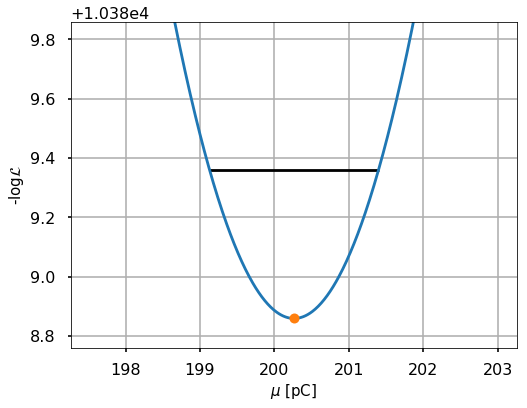
\includegraphics[width=0.6\linewidth]{figures/error.png}}
\caption{Erreur de $1\sigma$ obtenue pour l'exemple précédent de l'ajustement selon la méthode du maximum de vraisemblance.}
\label{fig:error}
\end{figure}






%%%%%%%%%%%%%%%%%%%%%%%%%%%%%%%%%%%%%%%%%%
% Description of the Experiments
%%%%%%%%%%%%%%%%%%%%%%%%%%%%%%%%%%%%%%%%%%

\section{Dispositif: Effet Tcherenkov par des électrons}

Cette manipulation a pour but la caractérisation d'un module optique (OM) développé pour l'expérience AMANDA. Afin d'étudier les propriétés de cet OM, vous devrez mettre au point le dispositif nécessaire à la prise de mesure. Après avoir pris connaissance avec le dispositif, vous serez ainsi amené à développer vous même la logique d'acquisition des données. Vous analyserez ensuite celles-ci grâce aux outils statistiques et informatiques que vous aurez vu en cours. \\

Cette manipulation utilise une source de radiation $\beta^+$ composée de Strontium $^{90}$Sr. Les électrons émis par la source traverse ensuite une plaque de quartz d'indice de réfraction  $n = 1.478$. Lors de leur passage, les électrons vont produire un rayonnement Tcherenkov qui pourra être détecté par l'OM. Dans ce dispositif, l'OM se trouve à une position fixe située à un angle de 45$^{\circ}$ par rapport à la direction d'émission des électrons. La source radioactive est combinée à un spectromètre qui va nous permettre de sélectionner l'énergie cinétique des électrons afin de récolter un maximum de rayonnement Tcherenkov dans l'OM. Pour déterminer l'intensité du courant à fournir au spectromètre pour obtenir des électrons de cette énergie, vous devrez d'abord résoudre l'exercice 2.\\

Une fois cette valeur trouvée, vous pouvez allumer le spectromètre. Celui-ci est calibré sur la partie descendante de la courbe d'hystérèse, il vous faudra donc respecter les conditions d'utilisation décrites ci-dessous.\\

\textbf{Mode d'emploi du spectromètre :}
\begin{quote}
    \begin{itemize}
        \item Démarrez à $I$ = 0 A
        \item Aller à saturation $I$ $\sim$ 2,6 A
        \item Descendre à la valeur $I_t$ désirée
    \end{itemize}
\end{quote}
\textbf{Remarque :} Si on veut changer $I_t$ pour une valeur plus petite, on descend vers cette valeur. En revanche, si on veut augmenter cette valeur, on doit recommencer le cycle d'hystérèse. 

\begin{figure}[!h]
    \centering
    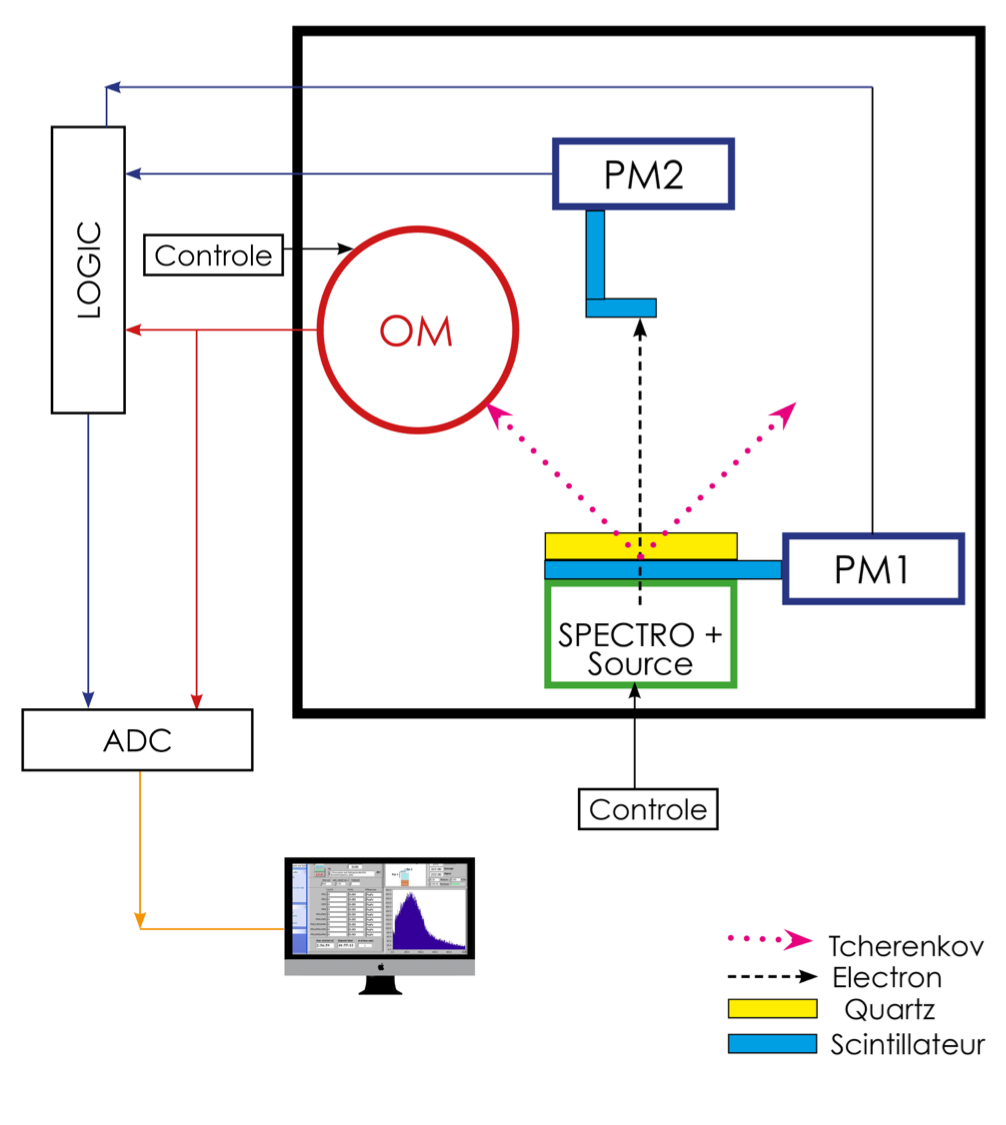
\includegraphics[width=0.5\textwidth]{figures/Dispositif_1.png}
    \caption{Dispositif expérimental de l'effet Tcherenkov produit par des électrons.}
    \label{fig:dispo1} 
\end{figure}

Dans ce dispositif, sont également présent 2 photo-multiplicateurs (PMs) chacun relié à un scintillateur. Le premier (PM1) est situé entre la source et la plaque de quartz et nous permet de vérifier qu'un électron a été émis par la source. Le second PM confirme que l'électron a bien traversé le quartz. Ces PMs ont donc pour but d'assurer que le signal détecté par l'OM est en coïncidence avec un électron qui a produit des photons Tcherenkov.


\subsection{Exercices Préparatoires}

\subsubsection{Exercice 1}
Sachant que l'OM est placé à un angle de $45^\circ$ par rapport à la direction d'émission des électrons ($m_\mathrm{e} = 0.511$\,MeV/$c^2$) de la source de strontium, à quel courant faut-il régler le spectromètre pour récolter un maximum de rayonnement Tcherenkov dans l'OM, sachant que l'indice de réfraction du quartz est de $1.478$?\\

Le graphique suivant vous donne la relation entre l'énergie cinétique des électrons et l'intensité du courant.

\begin{figure}[!h]
    \center{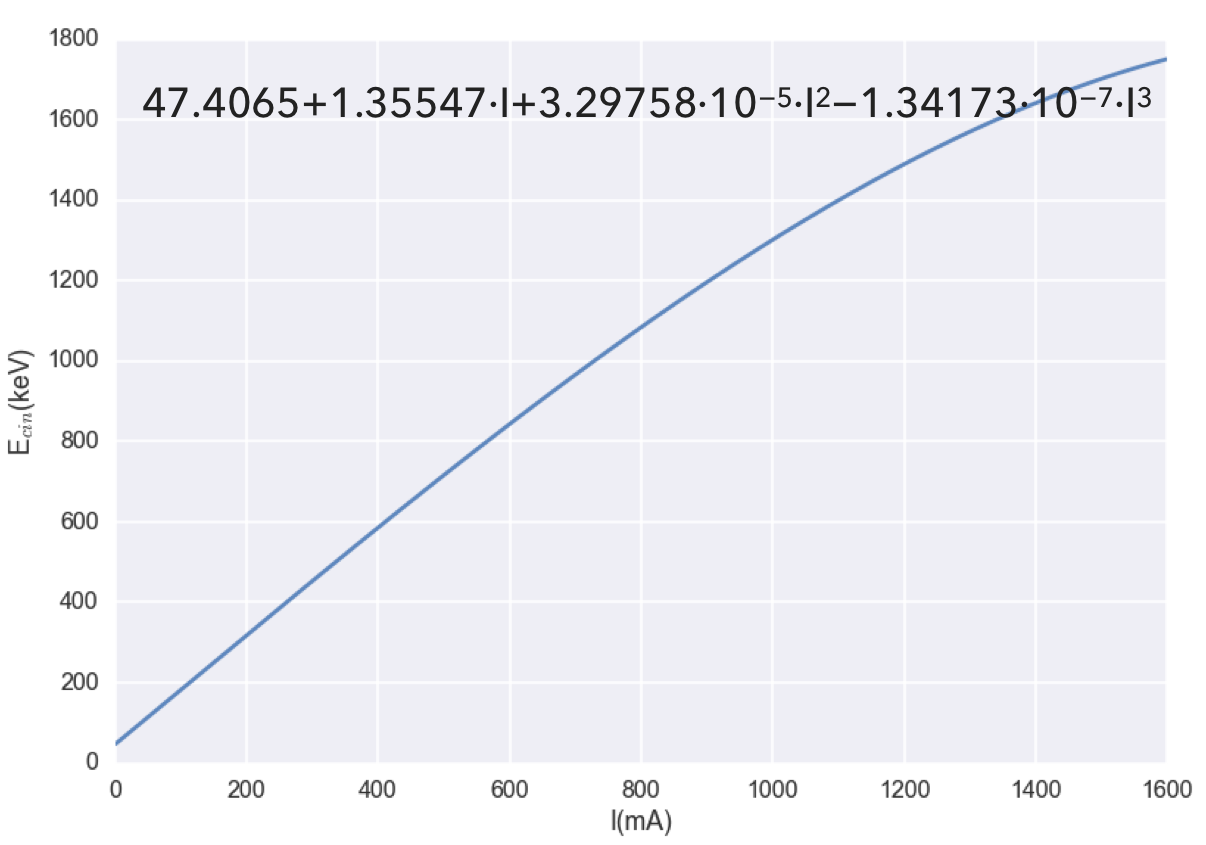
\includegraphics[width=0.5\textwidth]
    {figures/Relation_Ecin_I.png}}
    \caption{\label{fig:spectro} Relation entre l'intensité du courant fourni au spectromètre et l'énergie cinétique des électrons.}
\end{figure}

\ifthenelse{\boolean{showAdditional}}{
\begin{additional}
\begin{align*}
\beta &= \frac{1}{n\cos\Theta_\mathrm{c}} = 0.9568\\
 &= \frac{pc}{E}\\
 &= \frac{\sqrt{E^2-m_\mathrm{e}^2c^4}}{E}\\
 &\\
E &= \sqrt{\frac{m_\mathrm{e}^2c^4}{1 - \beta^2}} = 1.7575\,\mathrm{MeV}\\
E_\mathrm{cin}&=E- m_\mathrm{e}\\
 &= 1.247\,\mathrm{MeV} \\
&\Rightarrow \boxed{I \approx 950\,\mathrm{mA}} \\
\end{align*}
\end{additional}
}

\subsubsection{Exercice 2}
Calculer l'ordre de grandeur du nombre de photons émis entre $350$ et $500$\,nm par un électron de $1247$\,keV d'énergie cinétique traversant une fenêtre de quartz de 1\,mm d'épaisseur, sachant que pour ce domaine de longueurs d’onde, l'indice de réfraction du quartz varie de moins de 1\% et peut être considéré constant ($1.478$). Négliger la perte d'énergie de l'électron dans le quartz.\\ $\alpha = 1/137$

\ifthenelse{\boolean{showAdditional}}{
\begin{additional}
Formule de \emph{Frank-Tamm}:
\begin{align*}
\frac{\mathrm{d}N}{\mathrm{d}x} &= \int_{\lambda_0}^{\lambda_1} \frac{2\pi\alpha z^2}{\lambda^2} \sin^2\Theta_\mathrm{c} \mathrm{d}\lambda\\
&=\frac{\pi}{137}\int_{350\,\mathrm{nm}}^{500\,\mathrm{nm}}\frac{\mathrm{d}\lambda}{\lambda^2}\\
N&=\frac{\pi}{137}\cdot\left(\frac{1}{350\,\mathrm{nm}}-\frac{1}{500\,\mathrm{nm}}\right)\cdot1\,\mathrm{mm}\\
&=\boxed{19.65}
\end{align*}
\end{additional}
}

\subsubsection{Exercice 3}
En supposant que le diamètre du collimateur placé devant la photocathode de l'OM est de 6 cm et qu'il se trouve à 17\,cm de la fenêtre de quartz, combien de photoelectrons l'OM peut-il enregistrer par électron de la source, en supposant une transmittance $T$ de 90\% et sachant que l'efficacité quantique est de $\epsilon_\mathrm{q}=15\%$?

\ifthenelse{\boolean{showAdditional}}{
\begin{additional}
Avec $N_\mathrm{\gamma}^{\mathrm{quartz}}$ trouvé avant, on obtient:
\begin{align*}
N_{\mathrm{pe}} &= \epsilon_\mathrm{q} \cdot T \cdot N_\mathrm{\gamma}^{\mathrm{OM}}\\
 &= \epsilon_\mathrm{q} \cdot T \cdot \frac{6\,\mathrm{cm}}{2\pi \cdot 17\,\mathrm{cm} \cdot\sin\Theta_\mathrm{c}} \cdot N_\mathrm{\gamma}^{\mathrm{quartz}}\\
&= \boxed{3.58}
\end{align*}
\end{additional}
}


\subsection{Prise de mesure}

Pour cette manipulation, il vous est demandé de préparer le dispositif expérimental nécessaire à la prise de mesure. Cela implique, dans un premier temps, de :\\

\begin{center}
\fbox{
\begin{minipage}{0.75\textwidth}
\textbf{Se familiariser avec le dispositif :} 
\begin{quote}
\begin{itemize}
\item vérifier le signal des différents PMs et de l'OM
\item étudier l'efficacité des PMs
\item calibrer l'ADC
\item développer la logique d'acquisition de données
\item mesurer le bruit de fond
\end{itemize}
\end{quote}
\end{minipage}
}
\end{center}

\subsubsection{Vérification du dispositif}
Dans un premier temps, allumez votre dispositif et allumez la haute tension aux bornes des PM. Veillez ne pas changer la tension indiquée afin de ne pas endommager les PMs.\\

Après avoir calculé l'intensité du courant à fournir au spectromètre, allumer également celui-ci en suivant les instructions fournies précédement.\\

A l'aide de l'oscilloscope, vérifiez le signal provenant des différents photo-multiplicateurs (PMs) et de l'OM. Transformez ensuite votre signal analogue en signal digital à l'aide du discriminateur et observez celui-ci sur l'oscilloscope.
\subsubsection{Mesure de l'efficacité}

Il vous est ensuite demandé de mesurer l'efficacité d'un des PMs présents dans votre dispositif. Vous devrez faire cette mesure en faisant varier dans un premier temps le seuil du PM pour lequel vous mesurer l'efficacité. Une fois la valeur optimale du seuil trouvée, répétez le processus en faisant cette fois varier la tension appliquée sur le PM en question. Pour ces deux mesures, veillez également à mesurer le taux d'évènements détectés par le PM dont vous mesurez l'efficacité. Pour effectuer ces mesures, vous avez à votre disposition un scaler NIM. De quel PM allez-vous mesurer l'efficacité ?

\ifthenelse{\boolean{showAdditional}}{
\begin{additional}
\begin{itemize}
\item Mesure de l'efficacité de PM1
\item Logique : (PM1 \& PM2 \& OM) et (PM2 \& OM)
\item Mesure du rate de PM1
\end{itemize}
\end{additional}
}

\subsubsection{Calibration de l'ADC}

Nous allons à présent procéder à la calibration du convertisseur analogique-numérique (ADC ou Analogue-to-Digital Converter). En effet, l'ADC vous donne des valeurs en ADC channel, il vous faut donc connaître à quelle charge équivaut un ADC channel.\\

Pour cette calibration, il faut fournir une charge connue et constante à l'ADC. Pour cela, vous avez à votre disposition un générateur de courant continu. Comment allez-vous procéder ? 

\ifthenelse{\boolean{showAdditional}}{
\begin{additional}
\begin{itemize}
    \item Charge de l'ADC de l'ordre du pC $\to$ $Q\sim100$\,pC 
    \item Utilisation d'une résistance: $U = RI$ avec $R = 2.2$\,k$\mathrm{\Omega}$
    \item Sachant que $Q = I\mathrm{\Delta}t$, déterminer $\mathrm{\Delta}t$
    \item Le gate est ensuite créé à l'aide du dual-timer
\end{itemize}
\end{additional}
}

\subsubsection{Prise de données}

Afin de prendre les données nécessaires à la caractérisation de l'OM, nous devons réfléchir à la logique d'acquisition. Nous allons utiliser l'ADC que nous venons de calibrer et lui fournir le signal de l'OM ainsi qu'une porte logique (gate). Pour créer ce gate, nous avons besoin des modules logiques. Il nous faut réfléchir aux conditions dans lesquelles ont veut déclencher la prise de mesure. En d'autres termes, quand voulons nous considérer le signal de l'OM? \\

Une fois que vous avez déterminé cela, vous pouvez implémenter votre logique à l'aide des modules à votre disposition. Il vous faudra ensuite vérifier que le signal de l'OM et votre porte logique sont en coïncidence à l'aide de l'oscilloscope. Lorsque vous avez effectué cette vérification, reliez le gate et le signal de l'OM à l'ADC pour commencer acquisition.\\

\textbf{Remarque :} Ayant plus d'évènements, la prise de mesure pour cette manipulation est plus rapide. De ce fait, il vous sera demandé d'effectuer plusieurs mesures en faisant varier la tension. Faites un graphique du gain et de la résolution en fonction de la tension.\\

\ifthenelse{\boolean{showAdditional}}{
\begin{additional}
\begin{itemize}
\item \textbf{Gate :} PM1 \& PM2 \& OM
\item Faire passer le gate dans le dual-timer pour avoir des fenêtres de tailles constantes
\item Vérifier que l'OM est en même temps que le gate
\item Donner les deux infos à l'ADC et prendre les mesures
\item Prendre des mesures en fonction de la tension pour voir la variation de la position du pic de 1 pe
\end{itemize}
\end{additional}
}

\subsubsection{Mesure du bruit de fond}

Intéressons nous au bruit de fond présent dans cette manipulation. Nous voulons connaître le taux de fausses coïncidences, càd les cas où l'OM nous envois un signal qui n'est pas dû à un photon Tcherenkov alors que notre porte logique s'est déclenchée. \\

Dans un premier temps, il vous faut réfléchir à la manière dont vous pouvez implémenter la prise de mesure du bruit de fond. Une fois cette méthode mise en place, vous pouvez démarrer l'acquisition du bruit de fond. A l'aide de l'oscilloscope, pensez toutefois à vérifier que le signal de l'OM et votre gate arrivent en même temps à l'ADC.

\ifthenelse{\boolean{showAdditional}}{
\begin{additional}
\begin{itemize}
\item \textbf{Gate :} PM1 \& PM2 \& OM$_{\mathrm{couvert}}$
\item L'OM n'étant pas fixé au reste du dispositif, il est possible de le séparer physiquement à l'aide d'une couverture
\end{itemize}
\end{additional}
}

\subsection{Analyse de donn\'ees}

A présent, nous pouvons nous concentrer sur l'analyse des donn\'ees dans le but de caractériser l'OM.

En vous basant sur les données, vous devrez calculer:
\begin{center}
\fbox{
\begin{minipage}{0.75\textwidth}
\textbf{Dispositif muon :}
\begin{itemize}
\item le gain $G$ de l'OM,
\item la r\'esolution $\sigma_\mathrm{G}$ de l'OM,
\item le nombre moyen de photo-\'electrons $\langle n_{\mathrm{pe}}\rangle$ produit par trigger dans l'OM.
\end{itemize}
\end{minipage}
}
\end{center}

\ifthenelse{\boolean{showAdditional}}{
\begin{additional}
\textbf{Validation de la procedure d'adjustement:}\\
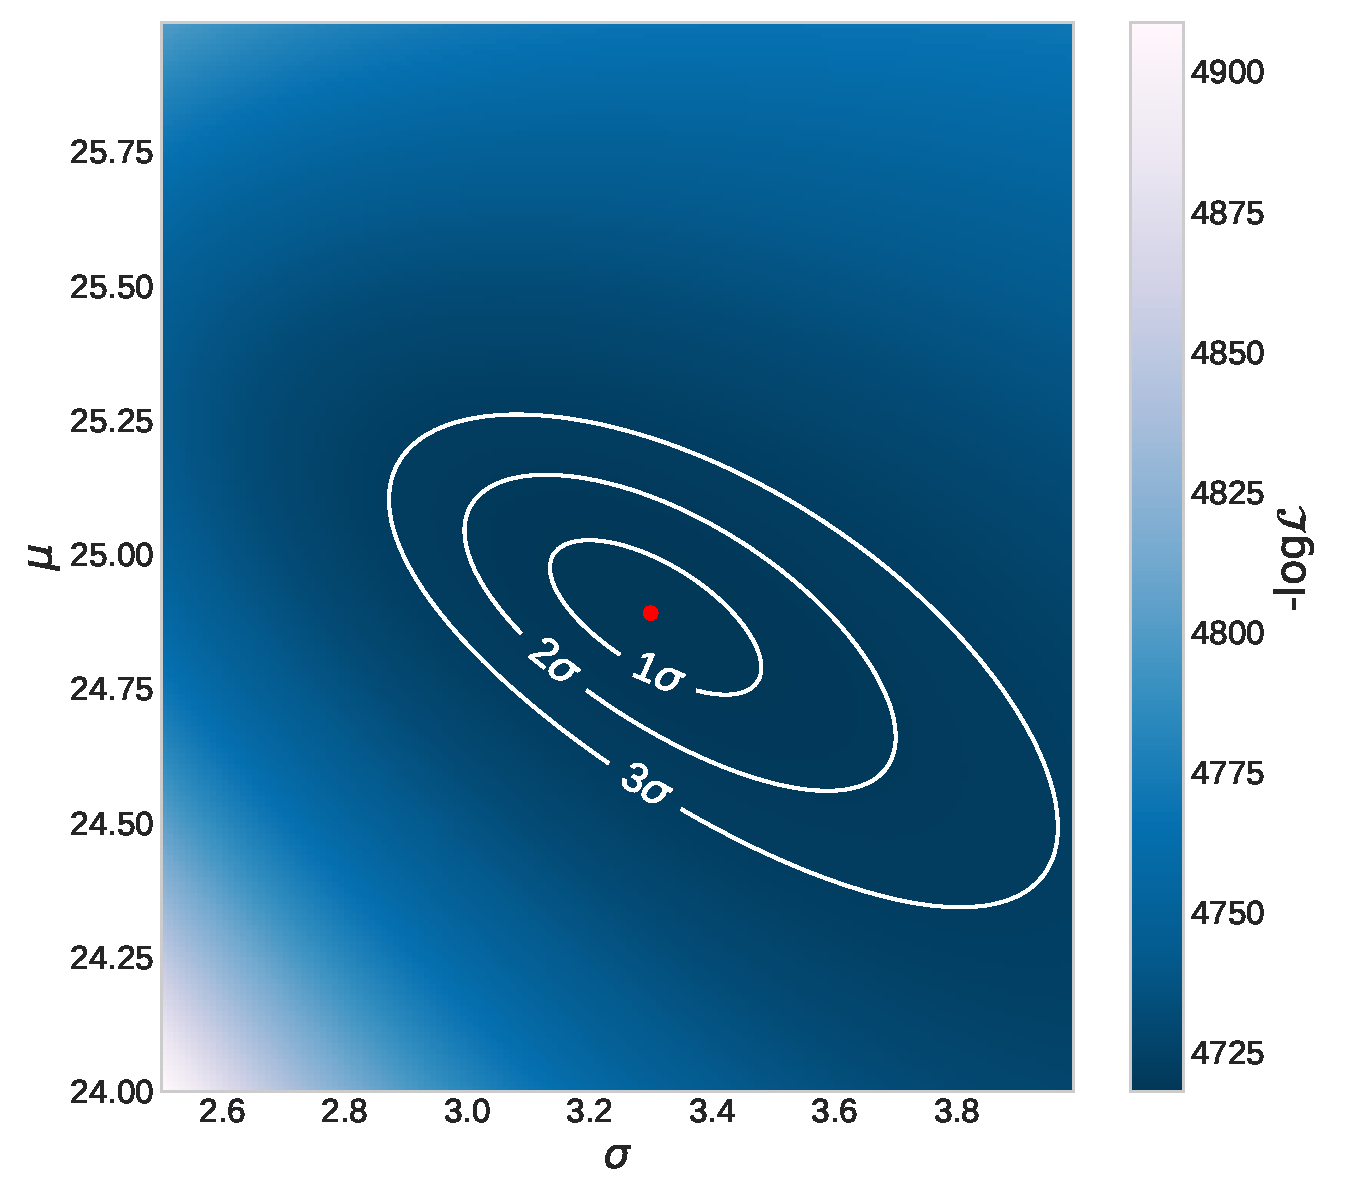
\includegraphics[width=0.45\textwidth]{exampleAnalysis/plots/Likelihood_MC.pdf}
\hfill 
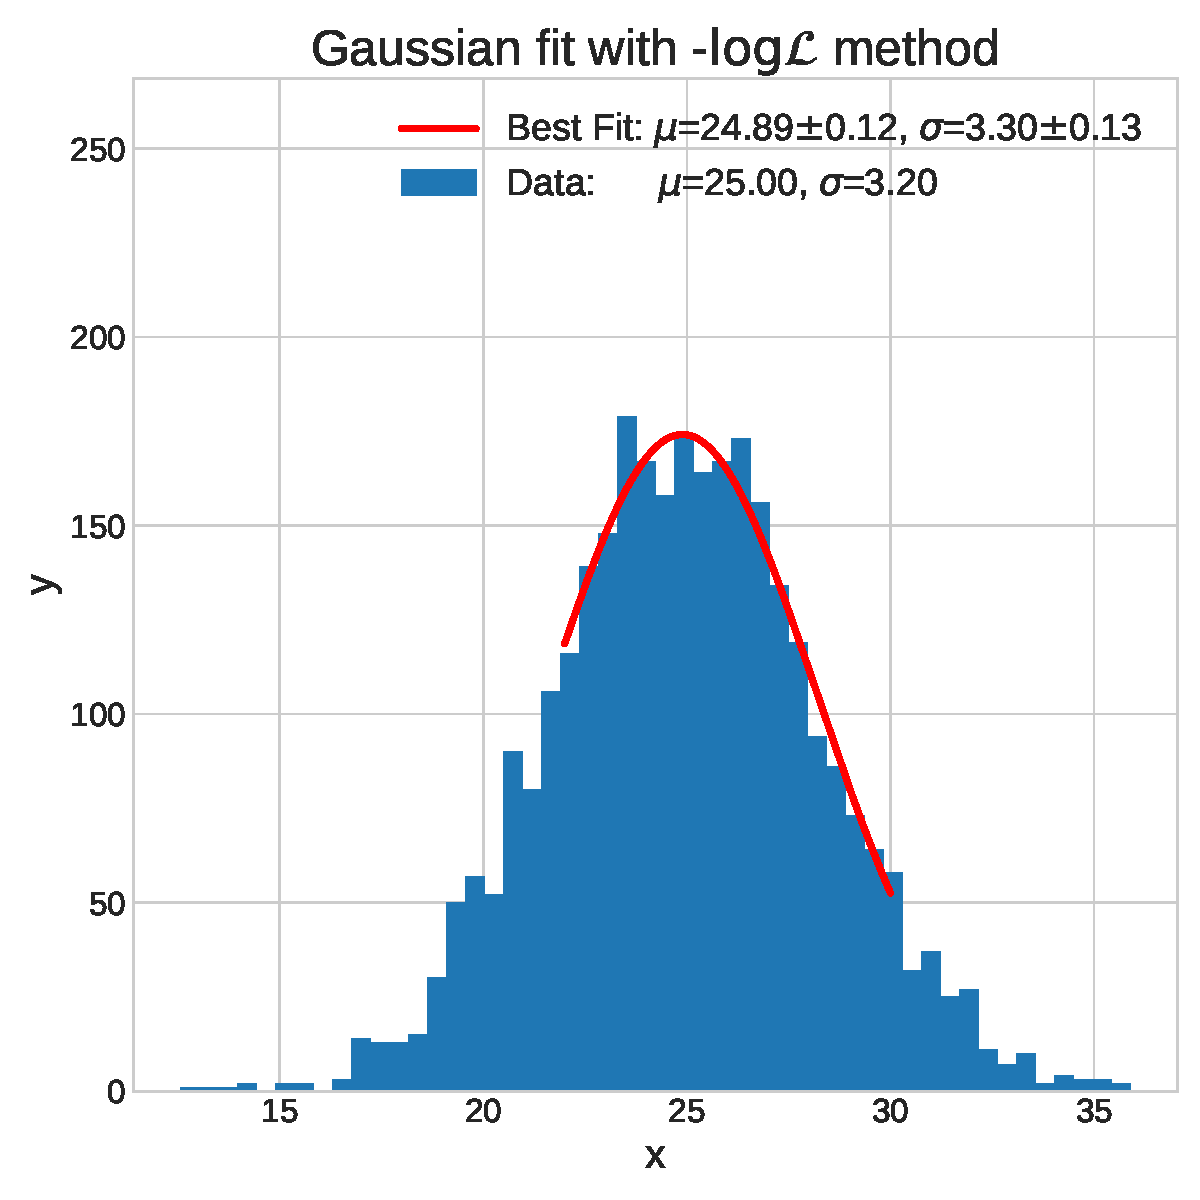
\includegraphics[width=0.45\textwidth]{exampleAnalysis/plots/LLH_Fit_MC.pdf}\\

\textbf{Ajustement des donn{\'e}es:}\\
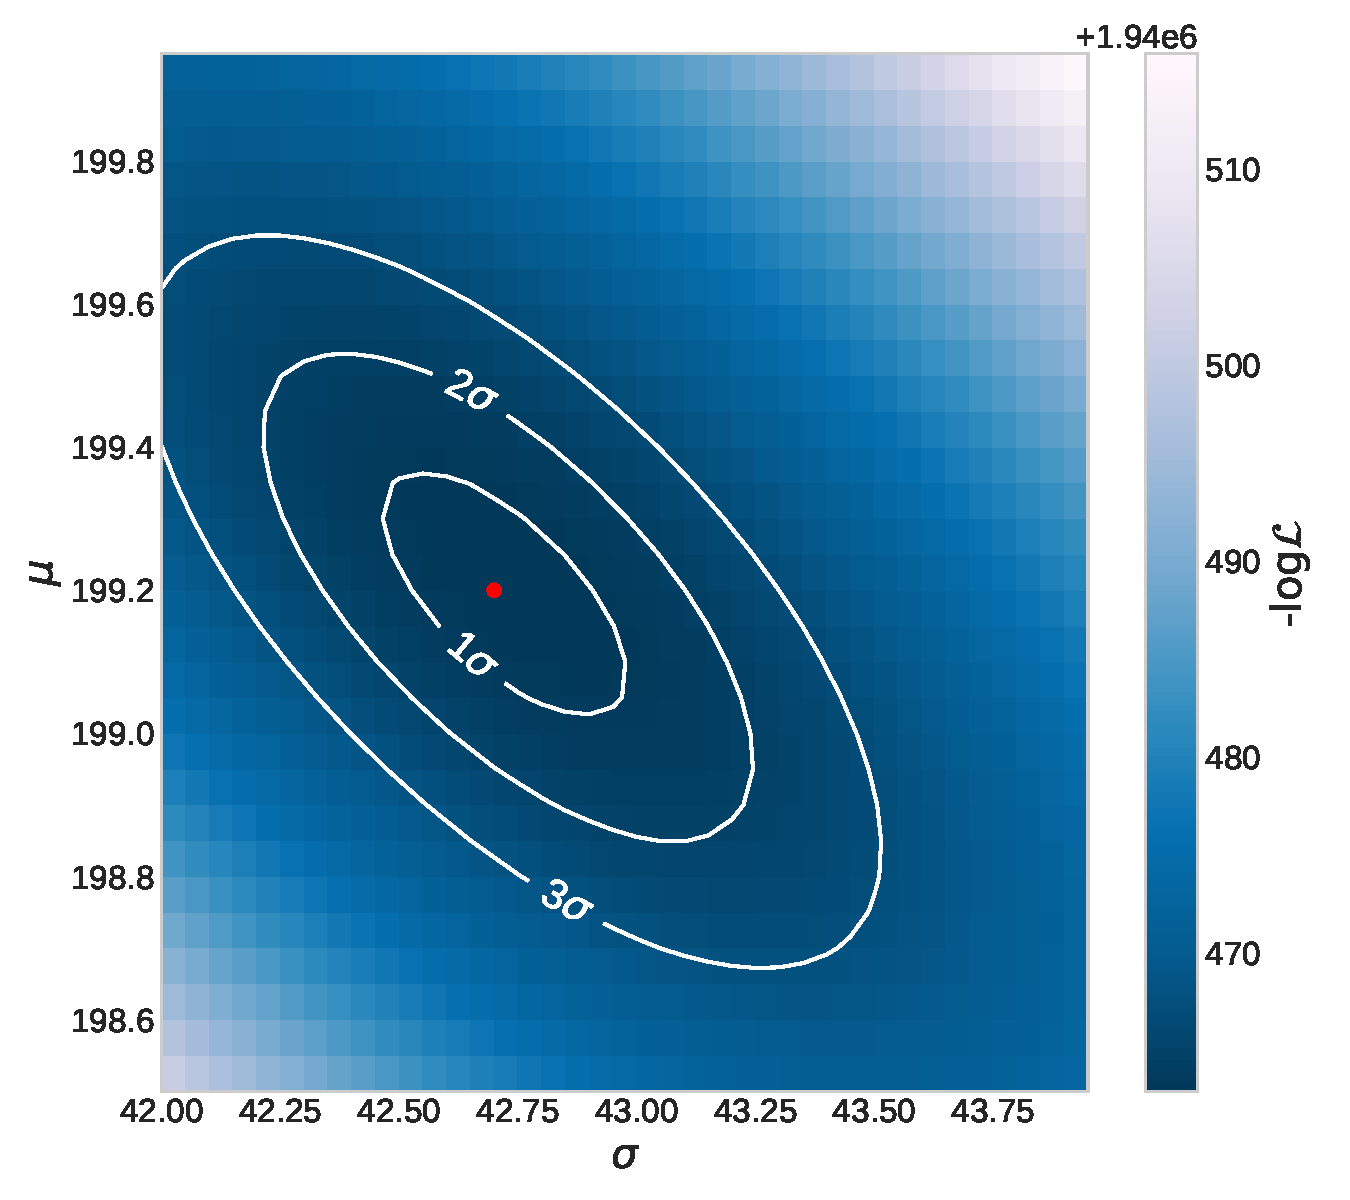
\includegraphics[width=0.45\textwidth]{exampleAnalysis/plots/Likelihood_Data_electron_VME.pdf}\hfill
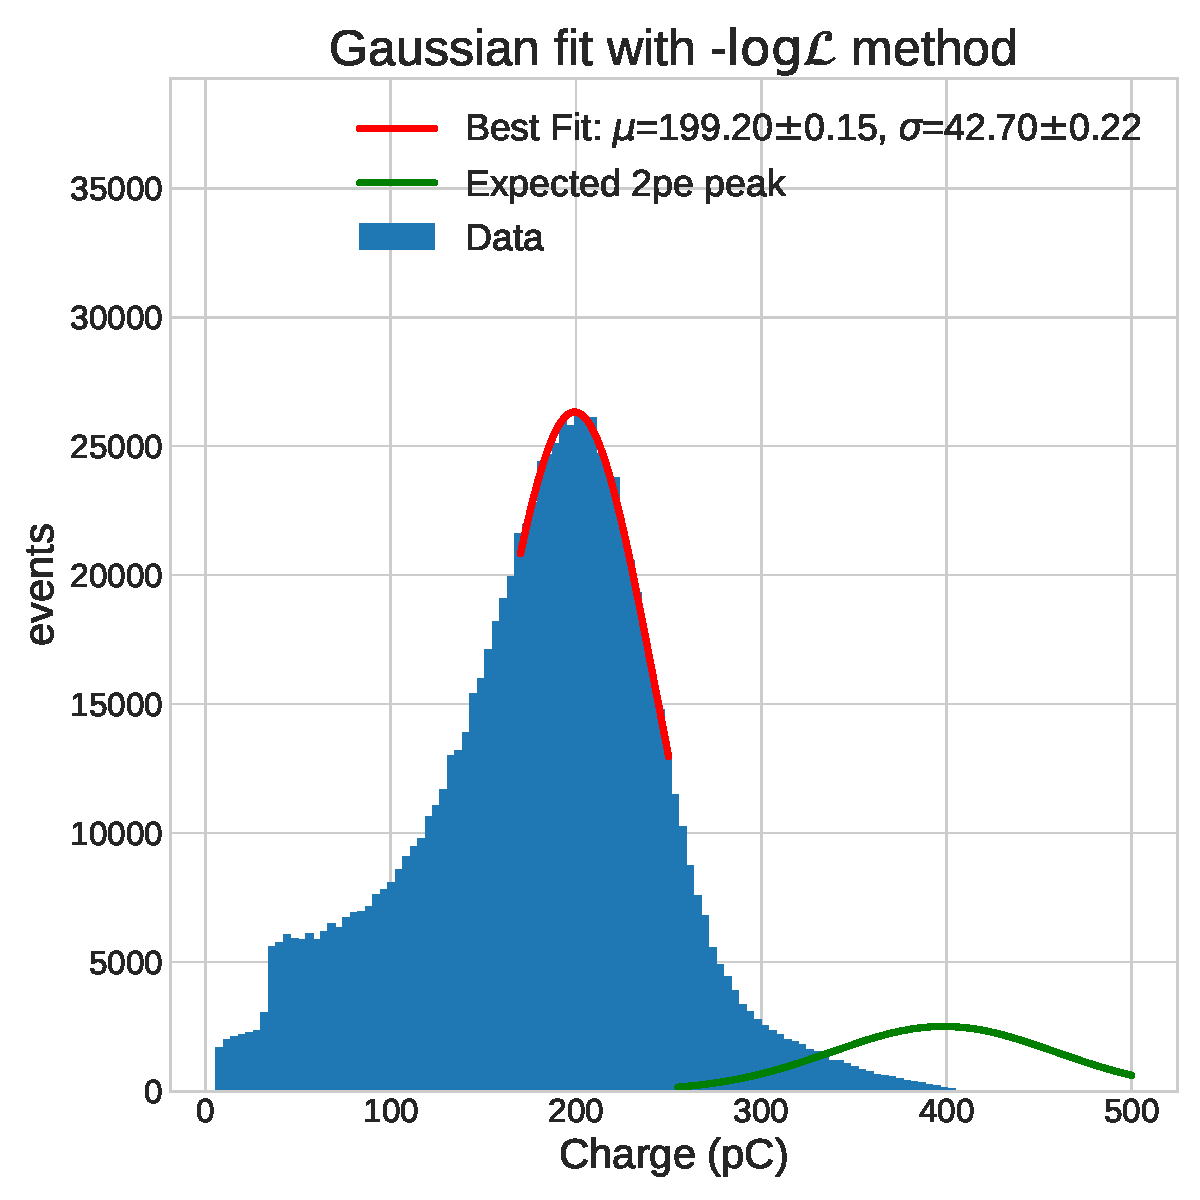
\includegraphics[width=0.45\textwidth]{exampleAnalysis/plots/LLH_Fit_electron_VME.pdf}
\begin{align*}
G &= \mu_{\text{best}}/e = 1242670 \\
\sigma_G &= \sigma_{\text{best}} / \mu_{\text{best}} = 21.44\%
\end{align*}
{\centering
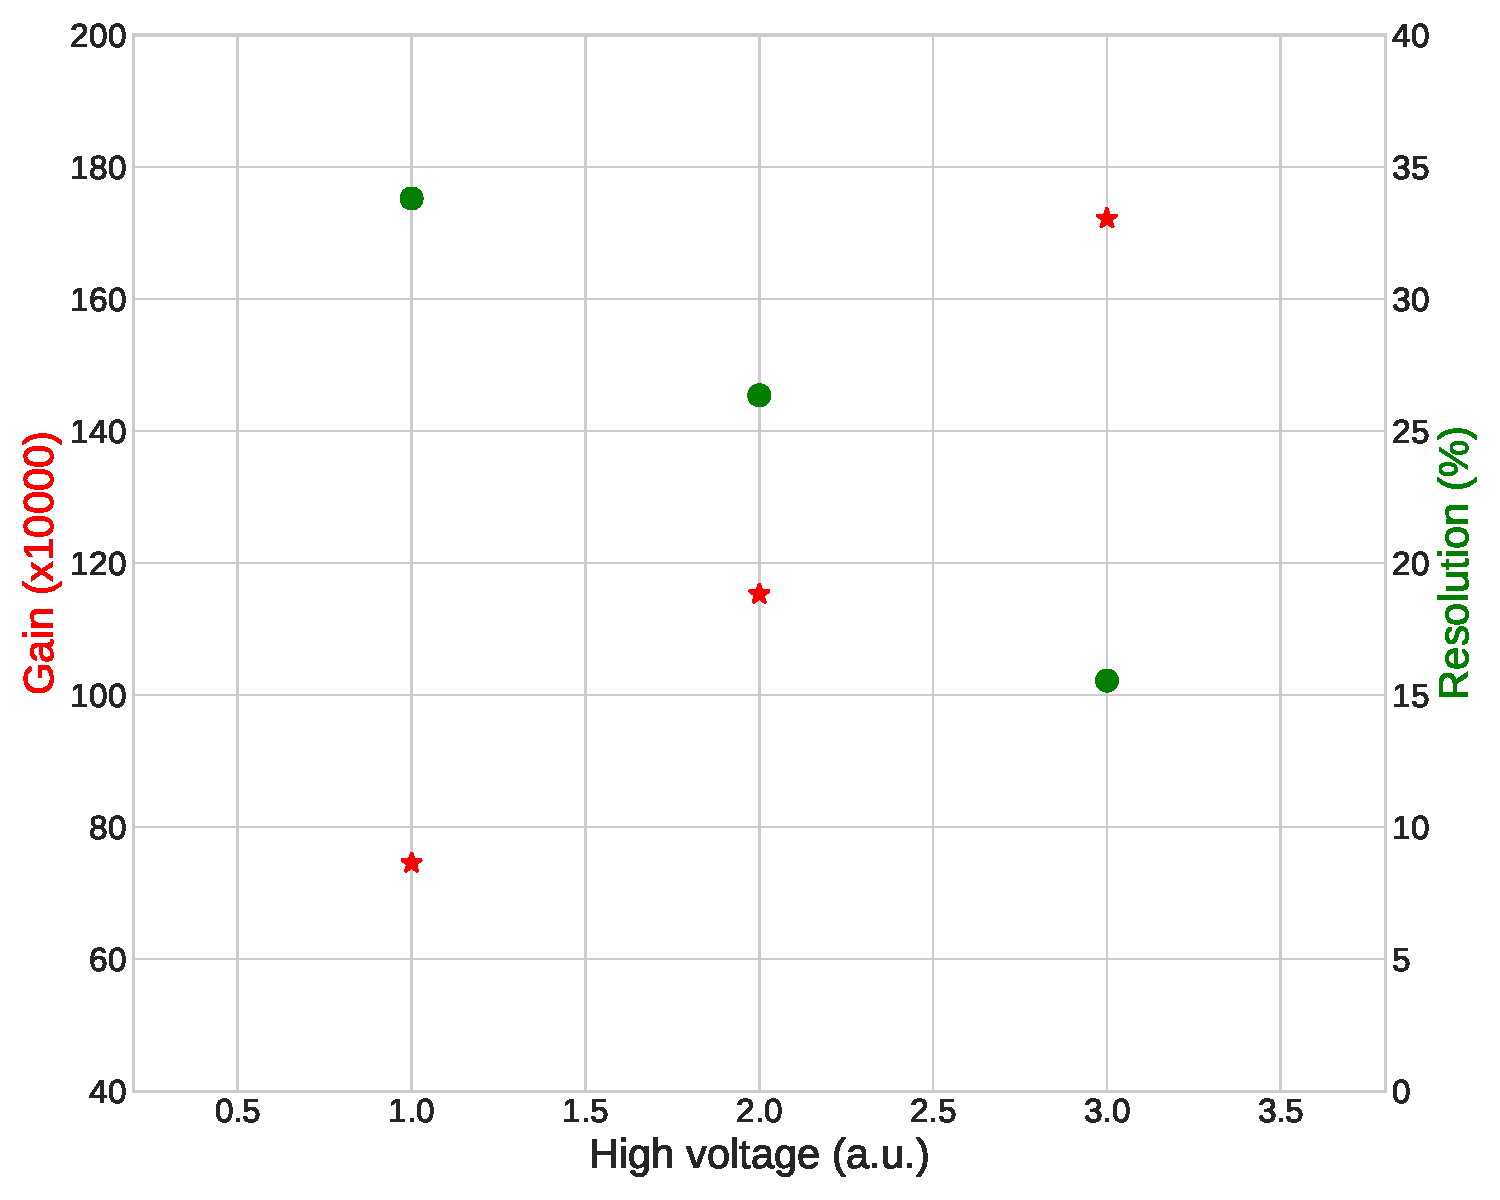
\includegraphics[width=0.7\textwidth]{exampleAnalysis/plots/Electron_Gain_Resolution_HV_VME.pdf}\\}
\end{additional}
}



\section{Dispositif: Effet Tcherenkov par des muons}
\label{sect:Tcherenkov_muon}

L'effet Tcherenkov survient lorsqu'une particule chargée se déplace plus vite que la vitesse de la lumière dans un milieu diélectrique. Ce phénomène résulte de la superposition cohérente d'onde électromagnétique suite à la polarisation du milieu par le passage de la particule chargée. Si la vitesse de la particule est supérieure au ratio $c/n$ (où $n$ est l'indice de réfraction et $c$ la vitesse de la lumière dans le vide), il y a formation d'un cône de lumière avec un angle de demi-ouverture $\Theta_c$ qui suit la relation:

\begin{equation}
    cos\Theta_c = \frac{1}{n\beta}
\end{equation}\\
où $\beta = v/c$, $v$ étant la vitesse de la particule dans le milieu. Le nombre de photons Tcherenkov émis par unité de longueur et de longeur d'onde est donné par la formule de Frank-Tamm:
\begin{equation}
     \frac{d^2N}{dx \, d\lambda} = \frac{2\pi \, \alpha}{\lambda^2} \; (1- \frac{1}{n^2 \, \beta^2} )
\end{equation}\\
avec $\alpha$ étant la constante de structure-fine. Comme le nombre de photons produits est inversement proportionnel à la longueur d'onde, la contribution des petites longueurs d'onde est plus importante.

Compte tenu de leur faible section efficace d'interaction, la détection des neutrinos nécessite un détecteur de grand volume. Cela est réalisé par les détecteurs Tcherenkov en déployant des photo-multiplicateurs (PMs) dans un volume de matériau diélectrique. Chaque PM est contenu dans une bulle de verre sous vide, l'ensemble étant appelé module optique (OM). AMANDA (Antarctic Muon and Neutrino Detector Array) est un télescope à neutrino localisé au Pôle Sud. Lors de sa phase finale, le détecteur était composé de 677 modules optiques (OMs) disposés sur 19 câbles. Ces modules retourne un signal analogique. Après 9 ans d'activité, AMANDA a été officiellement incorporé au détecteur IceCube en 2005. IceCube (figure~\ref{fig:IceCube}) est un détecteur Tcherenkov d'un kilomètre cube enterré dans la glace du Pôle Sud. Il a pour but principal la détection des neutrinos à haute énergie. IceCube est composé de 5160 modules optiques digitaux (DOMs ou Digital Optical Modules) placés sur 86 câbles. Pour constituer un vaste réseaux d'OMs, il nous faut connaître la réponse de chacun de ceux-ci.

\begin{figure}
    \center{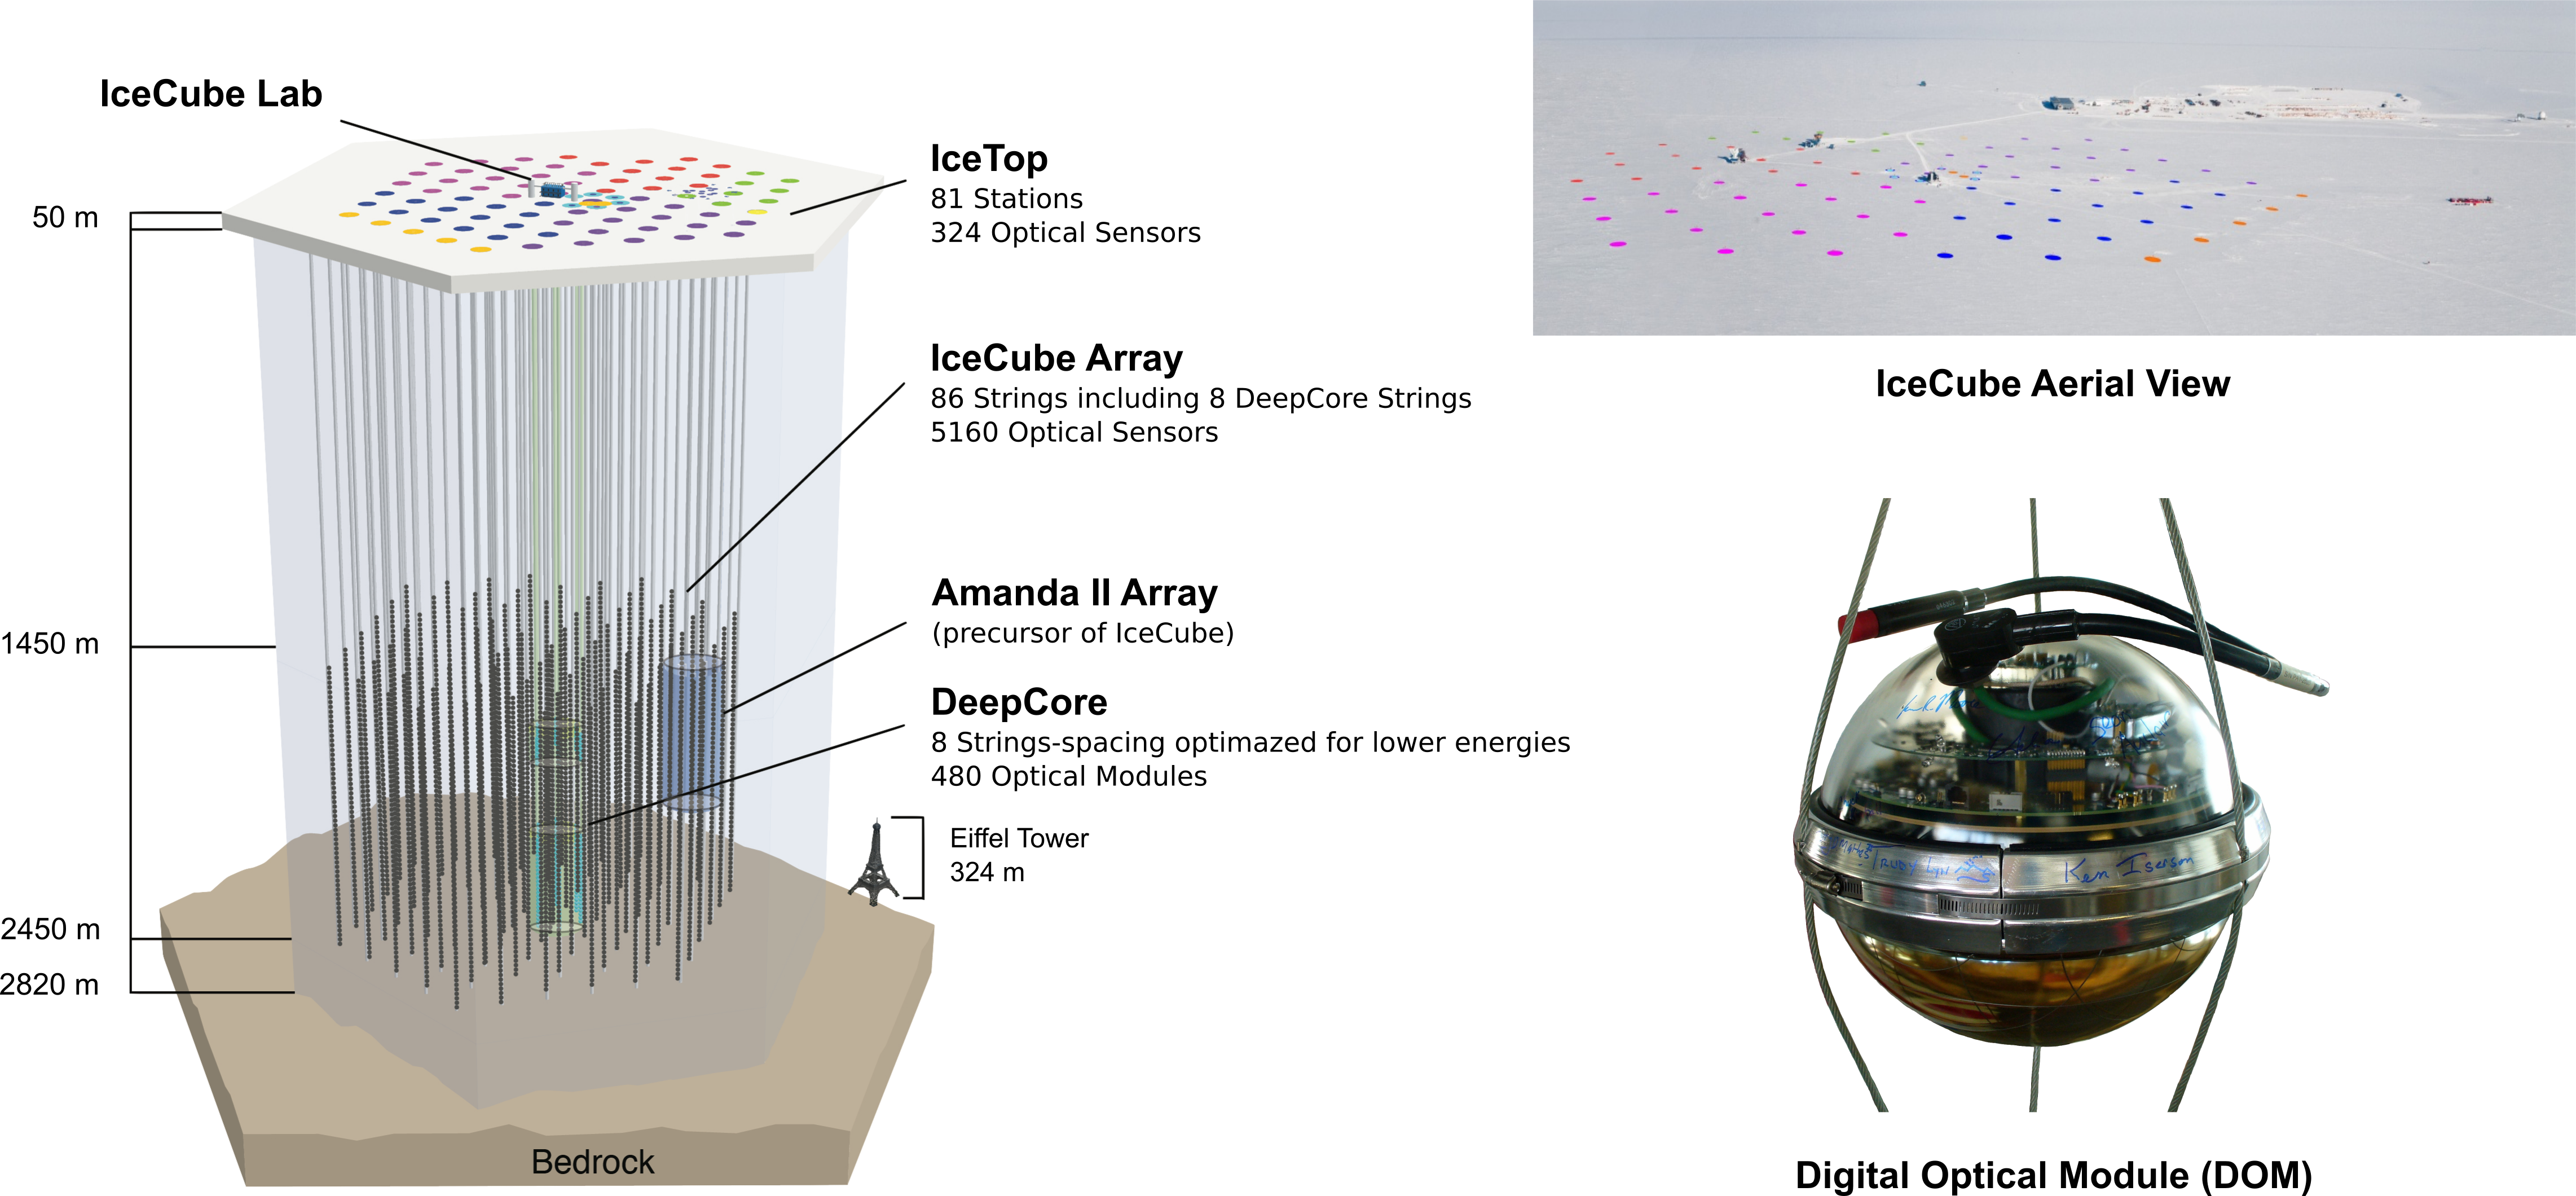
\includegraphics[width=0.8\textwidth]
    {figures/IceCube_Detector.png}}
    \caption{\label{fig:IceCube} Configuration du télescope à neutrinos IceCube.}
\end{figure}

Cette manipulation a pour but la caractérisation d'un module optique (OM) développé pour l'expérience AMANDA. Afin d'étudier les propriétés de cet OM, vous devrez mettre au point le dispositif nécessaire à la prise de mesure. Après avoir pris connaissance avec le dispositif, vous serez ainsi amené à développer vous même la logique d'acquisition des données. Vous analyserez ensuite les données recueillies grâce aux outils statistiques et informatiques que vous aurez vu en cours.

\subsection{Agenda du laboratoire}
\begin{tabular}{p{0.2\linewidth} p{0.8\linewidth}}
Lundi & - Prise de connaissance avec le matériel\newline
		- Vérification du signal analogique des PMs avec l'oscilloscope\newline
		- Implémentation de la table de vérité pour la logique d'acquisition ou trigger\newline
		- Mesure de l'efficacité\\ 

Mardi & - Calibration de l'ADC\newline
		- Préparation de l'acquisition de données\newline
		- Début de l'acquisition de données avec LabView\\ 

Mercredi & - Construction de la logique d'acquisition du bruit de fond\newline
		- Écriture de la table de vérité pour définir un événement du bruit\newline
		- Début de l'acquisition de données pour le bruit de fond\\ 

Jeudi et Vendredi & - Développement d'un programme de génération MC d'une distribution normale\newline
		- Développement des programmes d'analyse\newline
		- Dernier jour pour présenter les résultats des exercices\newline
		- Préparation de la présentation\\
\end{tabular} 

\subsection{Dispositif expérimental}

Pour cette manipulation, nous utilisons les muons atmosphériques afin d'obtenir l'émission Tcherenkov. Ce dispositif est composé de 4 scintillateurs chacun relié à un photo-multiplicateur (PM), d'un OM, une couche de plomb et d'un réservoir d'eau (voir figure \ref{fig:dispo2}). Ce réservoir forme un angle de 45$^{\circ}$ avec la verticale. Les trois premiers PMs (PM1, PM2 et PM3) assurent la direction verticale du muon incident. La présence d'une couche de plomb avant le PM3 nous permet également de vérifier que le muon est suffisamment énergétique pour produire le rayonnement Tcherenkov avec l'angle souhaité. Un 4ème PM est placé au dessus de l'OM et est utilisé comme veto. Puisque les muons sont produits en "paquets", appelés muon bundles, ce veto exclu les évènements de l'OM qui seraient produits par un second muon plutôt que par un photon Tcherenkov.

\begin{figure}
    \centering
	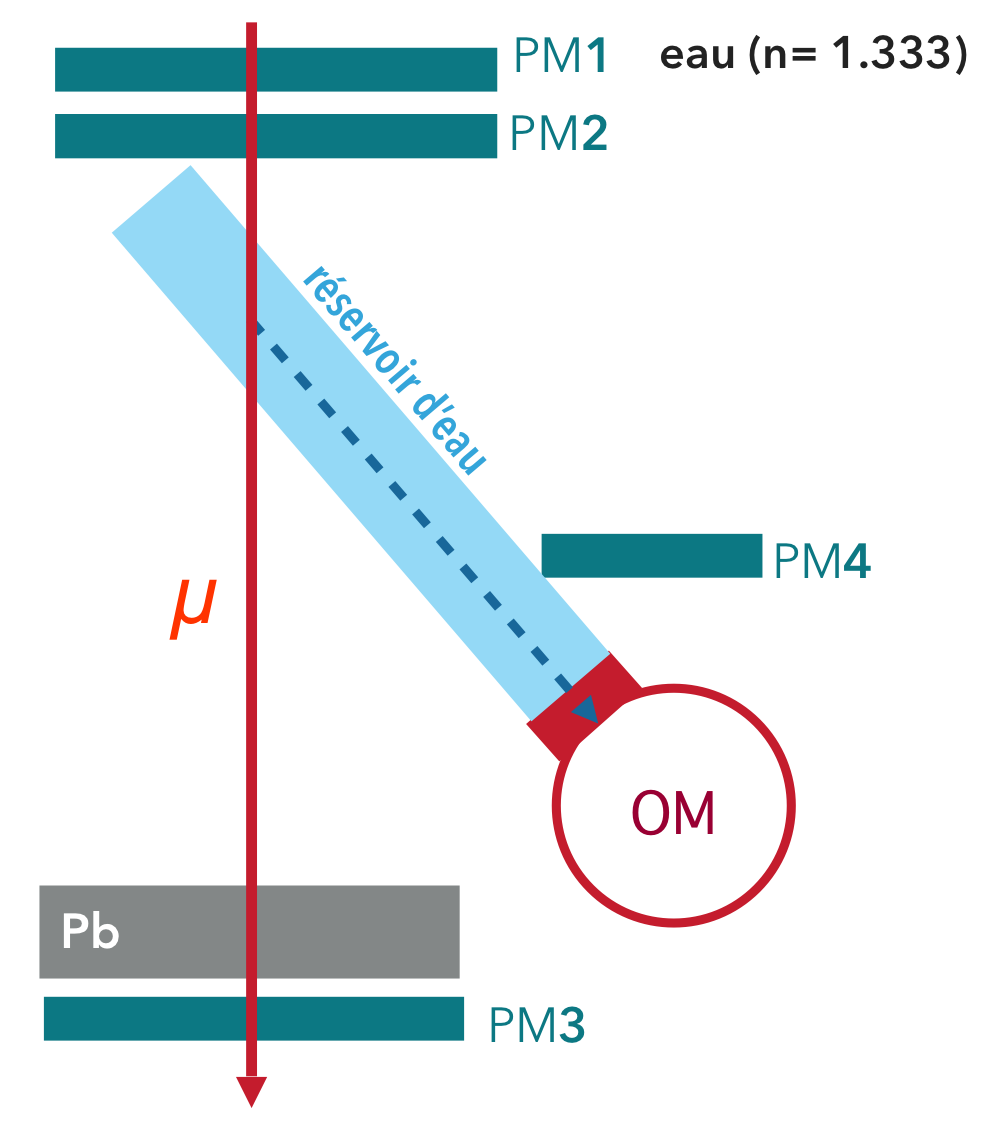
\includegraphics[width=0.5\textwidth]{figures/Dispositif_2.png}
    \caption{Dispositif expérimental de l'effet Tcherenkov produit par des muons.}
    \label{fig:dispo2} 
\end{figure}

\subsection{Exercices Pr\'eparatoires}

\subsubsection{Exercice 1}
Calculez quelle sera l'angle d'\'emission du rayonnement Tcherenkov \'emis dans l’eau par des muons ($m_\mathrm{\mu} = 0.106$\,GeV/$c^2$) de $1.5$\,GeV/$c$ de quantité de mouvement, sachant que l'indice de r\'efraction de l'eau \`a $20^\circ$C est $1.333$.

\ifthenelse{\boolean{showAdditional}}{
\begin{additional}
\begin{align*}
\begin{split}
\beta &= \frac{v}{c} = \frac{pc}{E}\\
 &= \frac{pc}{\sqrt{p^2c^2+m_\mathrm{\mu}^2c^4}}\\
 &= 0.9975\\
\end{split}
\quad
\begin{split}
\cos\Theta_\mathrm{c} &= \frac{1}{\beta n}\\
 \Theta_\mathrm{c} &= \arccos\frac{1}{0.9975\cdot1.33}\\
 &= \boxed{41.2^\circ} 
\end{split}
\end{align*}
\end{additional}
}

\subsubsection{Exercice 2}
Calculer l'ordre de grandeur du nombre de photons \'emis entre $350$ et $500$\,nm par un muon de $1.5$\,GeV/$c$ de quantité de mouvement traversant un réservoir d'eau de 10\,cm d'\'epaisseur. Pour ce domaine de longueurs d’onde, l'indice de r\'efraction d'eau varie de moins de 1\% et peut \^etre consid\'er\'e constant ($1.333$). N\'egliger la perte d'\'energie du muon dans l'eau.\\ $\alpha = 1/137$

\ifthenelse{\boolean{showAdditional}}{
\begin{additional}
Formule de \emph{Frank-Tamm}:
\begin{align*}
\frac{\mathrm{d}N}{\mathrm{d}x} &= \int_{\lambda_0}^{\lambda_1} \frac{2\pi\alpha z^2}{\lambda^2} \sin^2\Theta_\mathrm{c} \mathrm{d}\lambda\\
&=\frac{0.868\pi}{137}\int_{350\,\mathrm{nm}}^{500\,\mathrm{nm}}\frac{\mathrm{d}\lambda}{\lambda^2}\\
N&=\frac{0.868\pi}{137}\cdot\left(\frac{1}{350\,\mathrm{nm}}-\frac{1}{500\,\mathrm{nm}}\right)\cdot1\,\mathrm{cm}\\
&=\boxed{1706}
\end{align*}
\end{additional}
}

\subsubsection{Exercice 3}
Les photons Tcherenkov sont produits \`a 1\,m de l'OM, devant lequel se trouve un collimateur de 10\,cm de diam\`etre. Combien de photoélectrons l'OM peut-il enregistrer par muon, en supposant la transmittance $T$ \`a 90\%, l'efficacit\'e quantique est de $\epsilon_\mathrm{q}=15\%$? L'absorption de photons dans l'eau peut \^etre négligée, ainsi que la réflexion de photons au bord du réservoir.

\ifthenelse{\boolean{showAdditional}}{
\begin{additional}
Avec $N_\mathrm{\gamma}^{\mathrm{eau}}$ trouv\'e avant, on obtient:
\begin{align*}
N_{\mathrm{pe}} &= \epsilon_\mathrm{q} \cdot T \cdot N_\mathrm{\gamma}^{\mathrm{OM}}\\
 &= \epsilon_\mathrm{q} \cdot T \cdot \frac{10\,\mathrm{cm}}{2\pi \cdot 100\,\mathrm{cm} \cdot\sin\Theta_\mathrm{c}} \cdot N_\mathrm{\gamma}^{\mathrm{eau}}\\
&= \boxed{5.56}
\end{align*}
\end{additional}
}

\subsection{Prise de mesure}

Pour cette manipulation, il vous est demandé de préparer le dispositif expérimental nécessaire à la prise de mesure. Cela implique, dans un premier temps, de :\\

\begin{center}
\fbox{
\begin{minipage}{0.75\textwidth}
\textbf{Se familiariser avec le dispositif :} 
\begin{quote}
\begin{itemize}
\item vérifier le signal des différents PMs et de l'OM
\item étudier l'efficacité des PMs
\item calibrer l'ADC
\item développer la logique d'acquisition de données
\item mesurer le bruit de fond
\end{itemize}
\end{quote}
\end{minipage}
}
\end{center}

\subsubsection{Vérification du dispositif}
Dans un premier temps, allumez votre dispositif et allumez la haute tension aux bornes des PMs. Veillez ne pas changer la tension indiquée afin de ne pas endommager les PMs.\\
A l'aide de l'oscilloscope, vérifiez le signal provenant des différents photo-multiplicateurs (PMs) et de l'OM. Transformez ensuite votre signal analogue en signal digital à l'aide du discriminateur et observez celui-ci sur l'oscilloscope.

\subsubsection{Mesure de l'efficacité}

Il vous est ensuite demandé de mesurer l'efficacité d'un des PMs présents dans votre dispositif. Vous devrez faire cette mesure en faisant varier dans un premier temps le seuil du PM pour lequel vous mesurer l'efficacité. Une fois la valeur optimale du seuil trouvée, répétez le processus en faisant cette fois varier la tension appliquée sur le PM en question. Pour ces deux mesures, veillez également à mesurer le taux d'évènements détectés par le PM dont vous mesurez l'efficacité. Pour effectuer ces mesures, vous avez à votre disposition un scaler NIM. De quel PM allez-vous mesurer l'efficacité ?

\ifthenelse{\boolean{showAdditional}}{
\begin{additional}
\begin{itemize}
\item Mesure de l'efficacité de PM2
\item Logique : (PM1 \& PM2 \& PM3) et (PM1 \& PM3)
\item Mesure du rate de PM2
\end{itemize}
\end{additional}
}

\subsubsection{Calibration de l'ADC}

Nous allons à présent procéder à la calibration du convertisseur analogique-numérique (ADC ou Analogue-to-Digital Converter). En effet, l'ADC vous donne des valeurs en ADC channel, il vous faut donc connaître à quelle charge équivaut un ADC channel.

Pour cette calibration, il faut fournir une charge connue et constante à l'ADC. Pour cela, vous avez à votre disposition un générateur de courant continu. Comment allez-vous procéder ? 

\ifthenelse{\boolean{showAdditional}}{
\begin{additional}
\begin{itemize}
    \item Charge de l'ADC de l'ordre du pC $\to$ $Q\sim100$\,pC 
    \item Utilisation d'une résistance: $U = RI$ avec $R = 2.2$\,k$\mathrm{\Omega}$
    \item Sachant que $Q = I\mathrm{\Delta}t$, déterminer $\mathrm{\Delta}t$
    \item Le gate est ensuite créé à l'aide du dual-timer
\end{itemize}
\end{additional}
}

\subsubsection{Prise de données}

Afin de prendre les données nécessaires à la caractérisation de l'OM, nous devons réfléchir à la logique d'acquisition. Nous allons utiliser l'ADC que nous venons de calibrer et lui fournir le signal de l'OM ainsi qu'une porte logique (gate). Pour créer ce gate, nous avons besoin des modules logiques. Il nous faut réfléchir aux conditions dans lesquelles ont veut déclencher la prise de mesure. En d'autres termes, quand-est-ce que le signal de l'OM nous intéresse? Une fois que cela est clair, vous pouvez l'implémenter à l'aide des modules logiques. Il vous faudra ensuite vérifier que le signal de l'OM et votre porte logique sont en coïncidence à l'aide de l'oscilloscope. Lorsque vous avez effectué cette vérification, reliez le gate et le signal de l'OM à l'ADC pour commencer la prise de mesure.

\textbf{Attention :} Pour la manipulation utilisant les muons, veillez à changer le nom du fichier pour ne pas qu'il soit écrasé lors de la prise de mesure suivante.

\ifthenelse{\boolean{showAdditional}}{
\begin{additional}
\begin{itemize}
\item \textbf{Gate :} (PM1 \& PM2 \& PM3) \& (OM \& !PM4)
\item Faire passer le gate dans le dual-timer pour avoir des fenêtres de taille constante
\item Vérifier que l'OM est en même temps que le gate
\item On veut aussi le muon rate ($\sim 1$\,Hz) donc on passe (PM1 \& PM2 \& PM3) dans le scaler relié au PC
\item Donner le gate et le signal à l'ADC (taux de coïncidence $\sim 0.2$\,Hz) et commencez la prise de mesure
\end{itemize}
\end{additional}
}

\subsubsection{Mesure du bruit de fond}

Intéressons nous au bruit de fond présent dans votre manipulation. Nous voulons connaître le taux de fausses coïncidences, càd les cas où l'OM nous envoie un signal qui n'est pas dû à un photon Tcherenkov alors que notre porte logique s'est déclenchée.

Dans un premier temps, il vous faut réfléchir à la manière dont vous pouvez implémenter la prise de mesure du bruit de fond. Une fois cette méthode mise en place, vous pouvez démarrer l'acquisition du bruit de fond. A l'aide de l'oscilloscope, pensez toutefois à vérifier que le signal de l'OM et votre gate arrivent en même temps à l'ADC.

\ifthenelse{\boolean{showAdditional}}{
\begin{additional}
\begin{itemize} 
\item \textbf{Gate :} (PM1 \& PM2 \& PM3) \& (OM$_{\mathrm{delayed}}$) \& !(PM4)
\begin{quote}
    A l'aide d'un câble, on ajoute un délai de 50\,ns sur l'OM avant la logique\\
    Cela permet la mesure du taux de fausses coïncidences\\
    On obtient un taux très faible avec $\sim 1$ évènement par heure
\end{quote}

\item \textbf{Gate :} !(PM1 \& PM2 \& PM3) \& (OM) \& !(PM4)
\begin{quote}
    On s'intéresse ici à tous les évènements de l'OM qui ne sont pas dû à un photon Tcherenkov\\
    A partir de cela, on peut néanmoins calculer le taux de fausses coïncidences\\
    $R_{\mathrm{fc}} = 2 \cdot R_{\mathrm{mu}} \cdot R_{\mathrm{bf}} \cdot f $ \\
    où $R_{\mathrm{fc}}$ est le taux de fausse coïncidence, $R_{\mathrm{\mu}}$ le taux de muons et $f$ est la fenêtre de temps.
\end{quote}
\end{itemize}
\end{additional}
}

\subsection{Analyse de donn\'ees}

A présent, nous pouvons nous concentrer sur l'analyse des données dans le but de caractériser l'OM.

En vous basant sur les données, vous devrez calculer:\\
\begin{center}
\fbox{
\begin{minipage}{0.75\textwidth}
\textbf{Dispositif muon :}
\begin{itemize}
\item le gain $G$ de l'OM,
\item la r\'esolution $\sigma_\mathrm{G}$ de l'OM,
\item le nombre moyen de photo-\'electrons $\langle n_{\mathrm{pe}}\rangle$ produit par trigger dans l'OM.
\end{itemize}
\end{minipage}
}
\end{center}

\ifthenelse{\boolean{showAdditional}}{
\begin{additional}
\textbf{Validation de la procedure d'adjustement:}\\
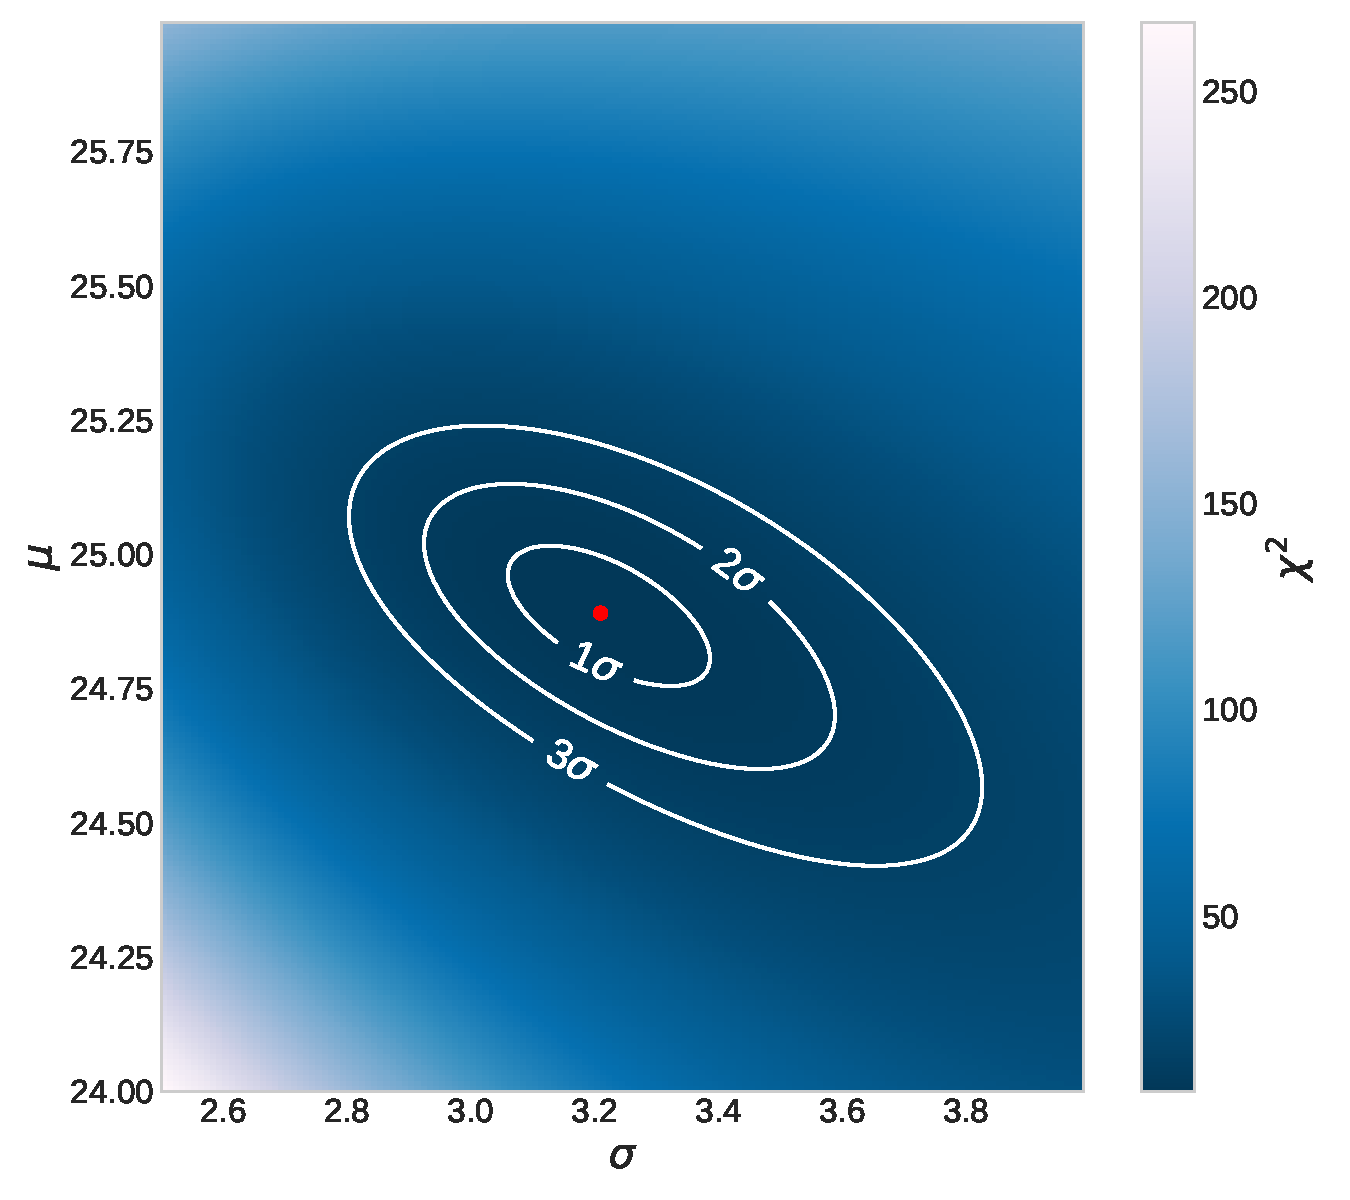
\includegraphics[width=0.45\textwidth]{exampleAnalysis/plots/Chi2_MC.pdf}
\hfill 
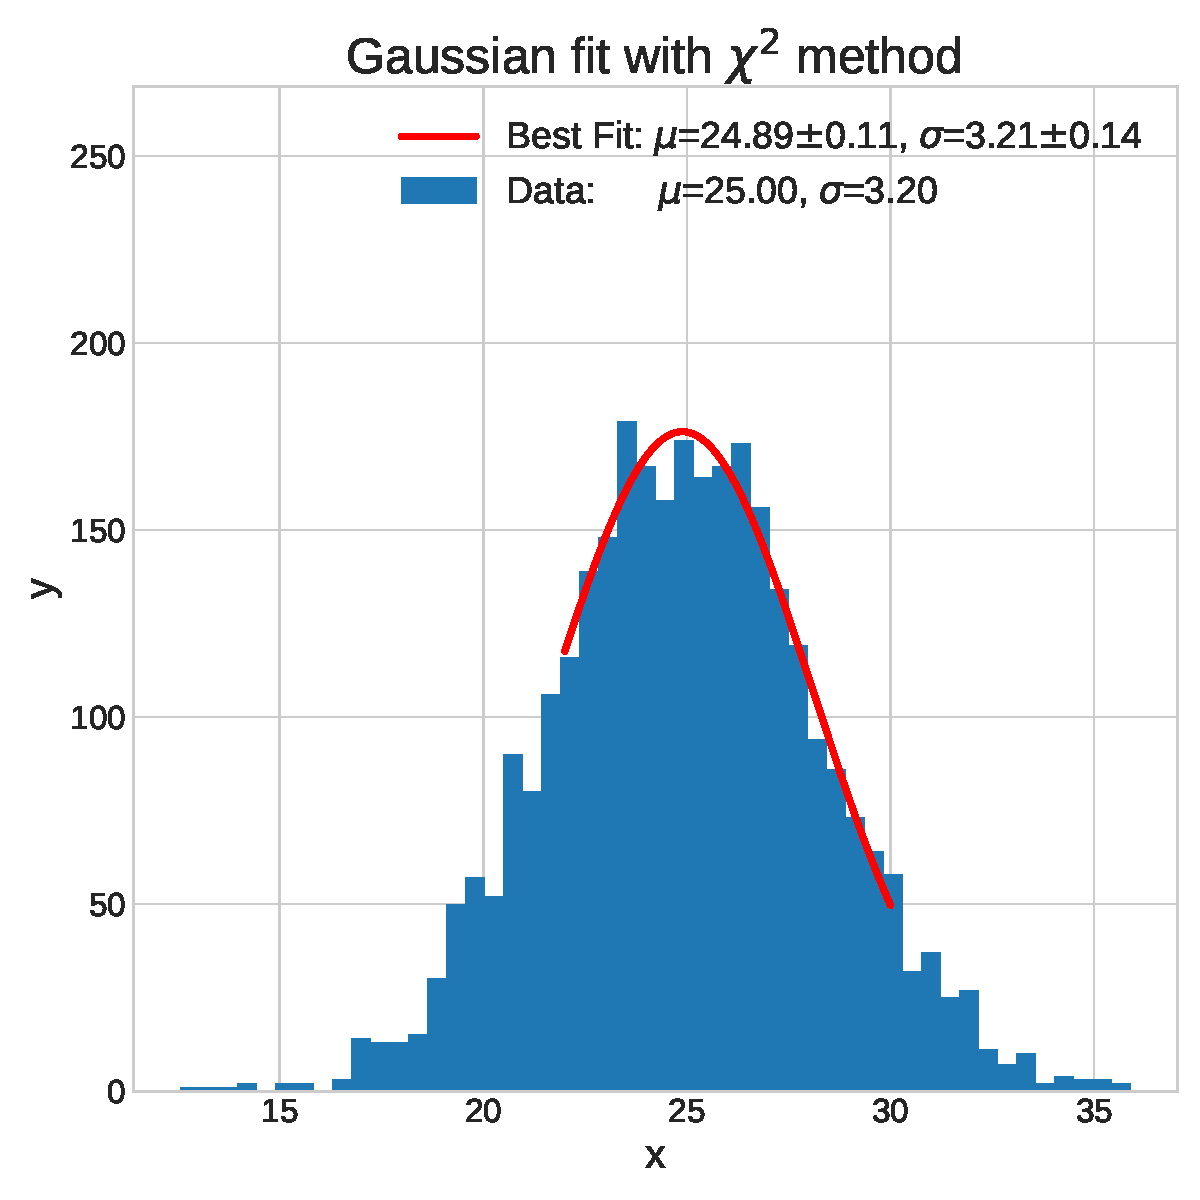
\includegraphics[width=0.45\textwidth]{exampleAnalysis/plots/Chi2_fit_MC.pdf}\\

\textbf{Ajustement des donn{\'e}es:}\\
\begin{align*}
G &= \mu_{\text{best}}/e = ... \\
\sigma_G &= \sigma_{\text{best}} / \mu_{\text{best}} = ...\%\\
\langle n_{\mathrm{pe}}\rangle &= ...
\end{align*}
\end{additional}
}



\section{Dispositif: Temps de vie de muons}

\section{Dispositif: L'arche cosmique}

\end{document}
